\documentclass{scrreprt}
\usepackage{array}
\usepackage{graphicx}
\usepackage{listings}
\usepackage{underscore}
\usepackage[bookmarks=true]{hyperref}
\usepackage[utf8]{inputenc}
\usepackage{float}
\usepackage[french]{babel}
\hypersetup{
    bookmarks=false,    % show bookmarks bar
    pdftitle={rapport_TP1_Lambolez_Petit},    % title
    pdfauthor={Théodore Lambolez, Maximilien Petit},                     % author
    pdfsubject={TeX and LaTeX},                        % subject of the document
    pdfkeywords={TeX, LaTeX, graphics, images}, % list of keywords
    colorlinks=true,       % false: boxed links; true: colored links
    linkcolor=blue,       % color of internal links
    citecolor=black,       % color of links to bibliography
    filecolor=black,        % color of file links
    urlcolor=black,        % color of external links
    linktoc=page            % only page is linked
}
\def\myversion{1.0}
\date{}
%\title
\usepackage{hyperref}
\begin{document}
\begin{figure}
   \begin{minipage}[c]{.46\linewidth}
      
\includegraphics[scale=0.3]{images/telecom.png}
   \end{minipage} \hfill
   \begin{minipage}[c]{.46\linewidth}
      
\includegraphics[scale=1.9]{images/lorraine.jpg}
   \end{minipage}
\end{figure}
\begin{flushright}
    \rule{15cm}{5pt}
    \vskip1cm
\end{flushright}
\begin{center}
	\vspace{3cm}
	\fbox{
	\begin{minipage}{0.9\textwidth}
        	\Huge{
			\textbf{
			\begin{center}
				Rapport \\Travaux Pratiques 1
				\vspace{0.5cm}
			\end{center}
			}
		}
	\end{minipage}
	}
\end{center}
\begin{flushright}
        \vspace{5cm}
	\huge{
        \textbf{
	Ecrit par \\
	\vspace{0,875cm}
	\href{mailto:theodore.lambolez@telecomnancy.eu}{Théodore Lambolez} \\
	\href{mailto:maximilien.petit@telecomnancy.eu}{Maximilien Petit}\\
	}
	}
        \vspace{0,5cm}
        \large{
	\textbf{
	\today\\
	}	
	}
\end{flushright}

\tableofcontents

\chapter{Première partie}
\addcontentsline{toc}{chapter}{Première partie}

\begin{center}
\large{
\textbf{Caractérisation d’images et traitements au niveau du pixel.}}
\end{center}

\section{Caractérisation d'une image}
\addcontentsline{toc}{section}{Caractérisation d'une image}

Dans cette première section, nous aborderons la caractérisations de quatres images : Connect_OK, Connect_L,
Connect_D et PNCN 256. 	

\begin{center}
\begin{figure}[!h]
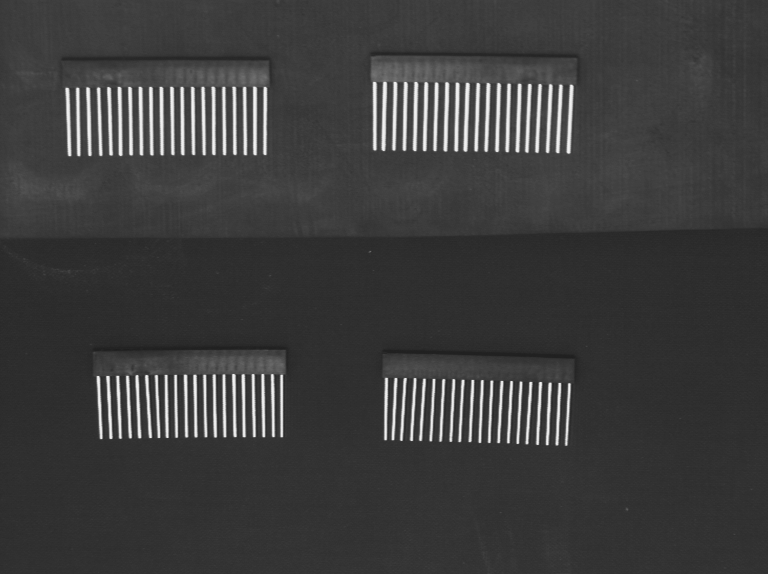
\includegraphics[scale=0.5]{images/ConnectOK.png}\hfill
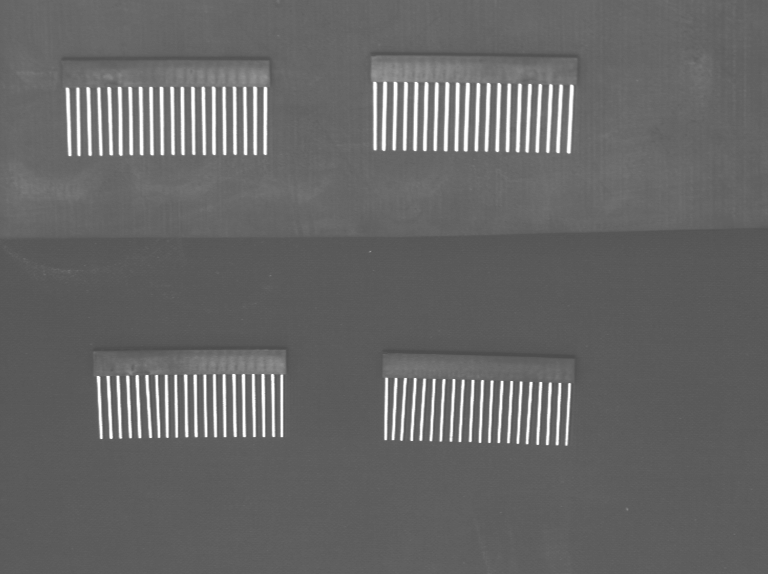
\includegraphics[scale=0.5]{images/ConnectL.png}\hfill
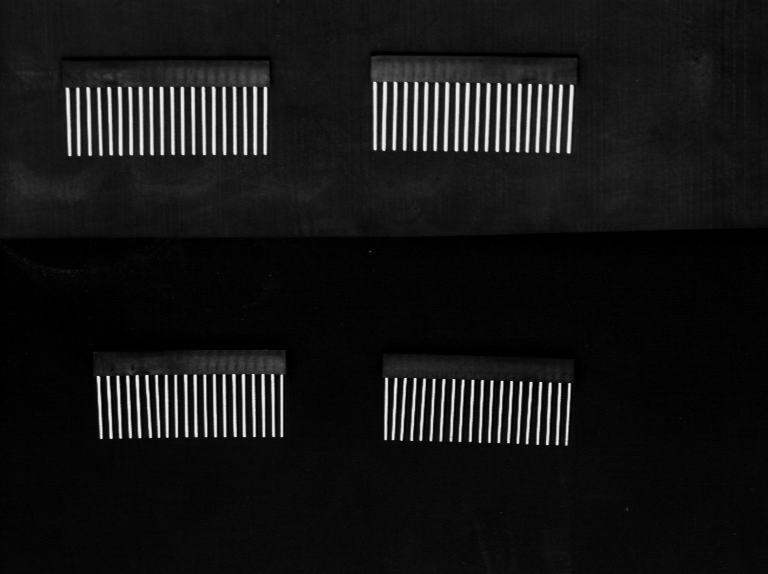
\includegraphics[scale=0.5]{images/ConnectD.png}
\caption{Connect Ok L D }
\end{figure}
\begin{figure}[!h]
\centering
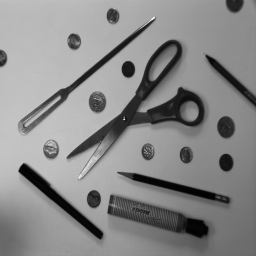
\includegraphics[scale=0.6]{images/PNCN256.png}
\caption{PNCN 256}
\end{figure}
\end{center}

\newpage
Tout d'abord, les images étant en niveaux de gris, nous avons commencé par effectuer les histogrammes des images de la figure 1.1. 
Sur cette figure sont présents l'histogramme de Connect_OK en bleu, de Connect_L en rouge et de Connect_D en vert. 
On constate de manière générale, que l'histogramme de la version "light" est décalé vers les niveaux de gris élevés par rapport
à l'histogramme de la version "OK" contrairement à celui de la version "dark" qui est décalé vers les niveaux de gris plus faibles.
Cela nous indique que l'image version "light" a été prise avec une forte luminosité comparé à celle lors de la prise de l'image "OK", 
contrairement à l'image version "dark" qui a été prise, quant à elle, avec une faible luminosité.
Grâce à l'outil Threshold, on a pu évaluer des encadrements de niveaux de gris pour chaque partie de ces images (voir table 1.1).
 
\begin{figure}[!h]
\centering
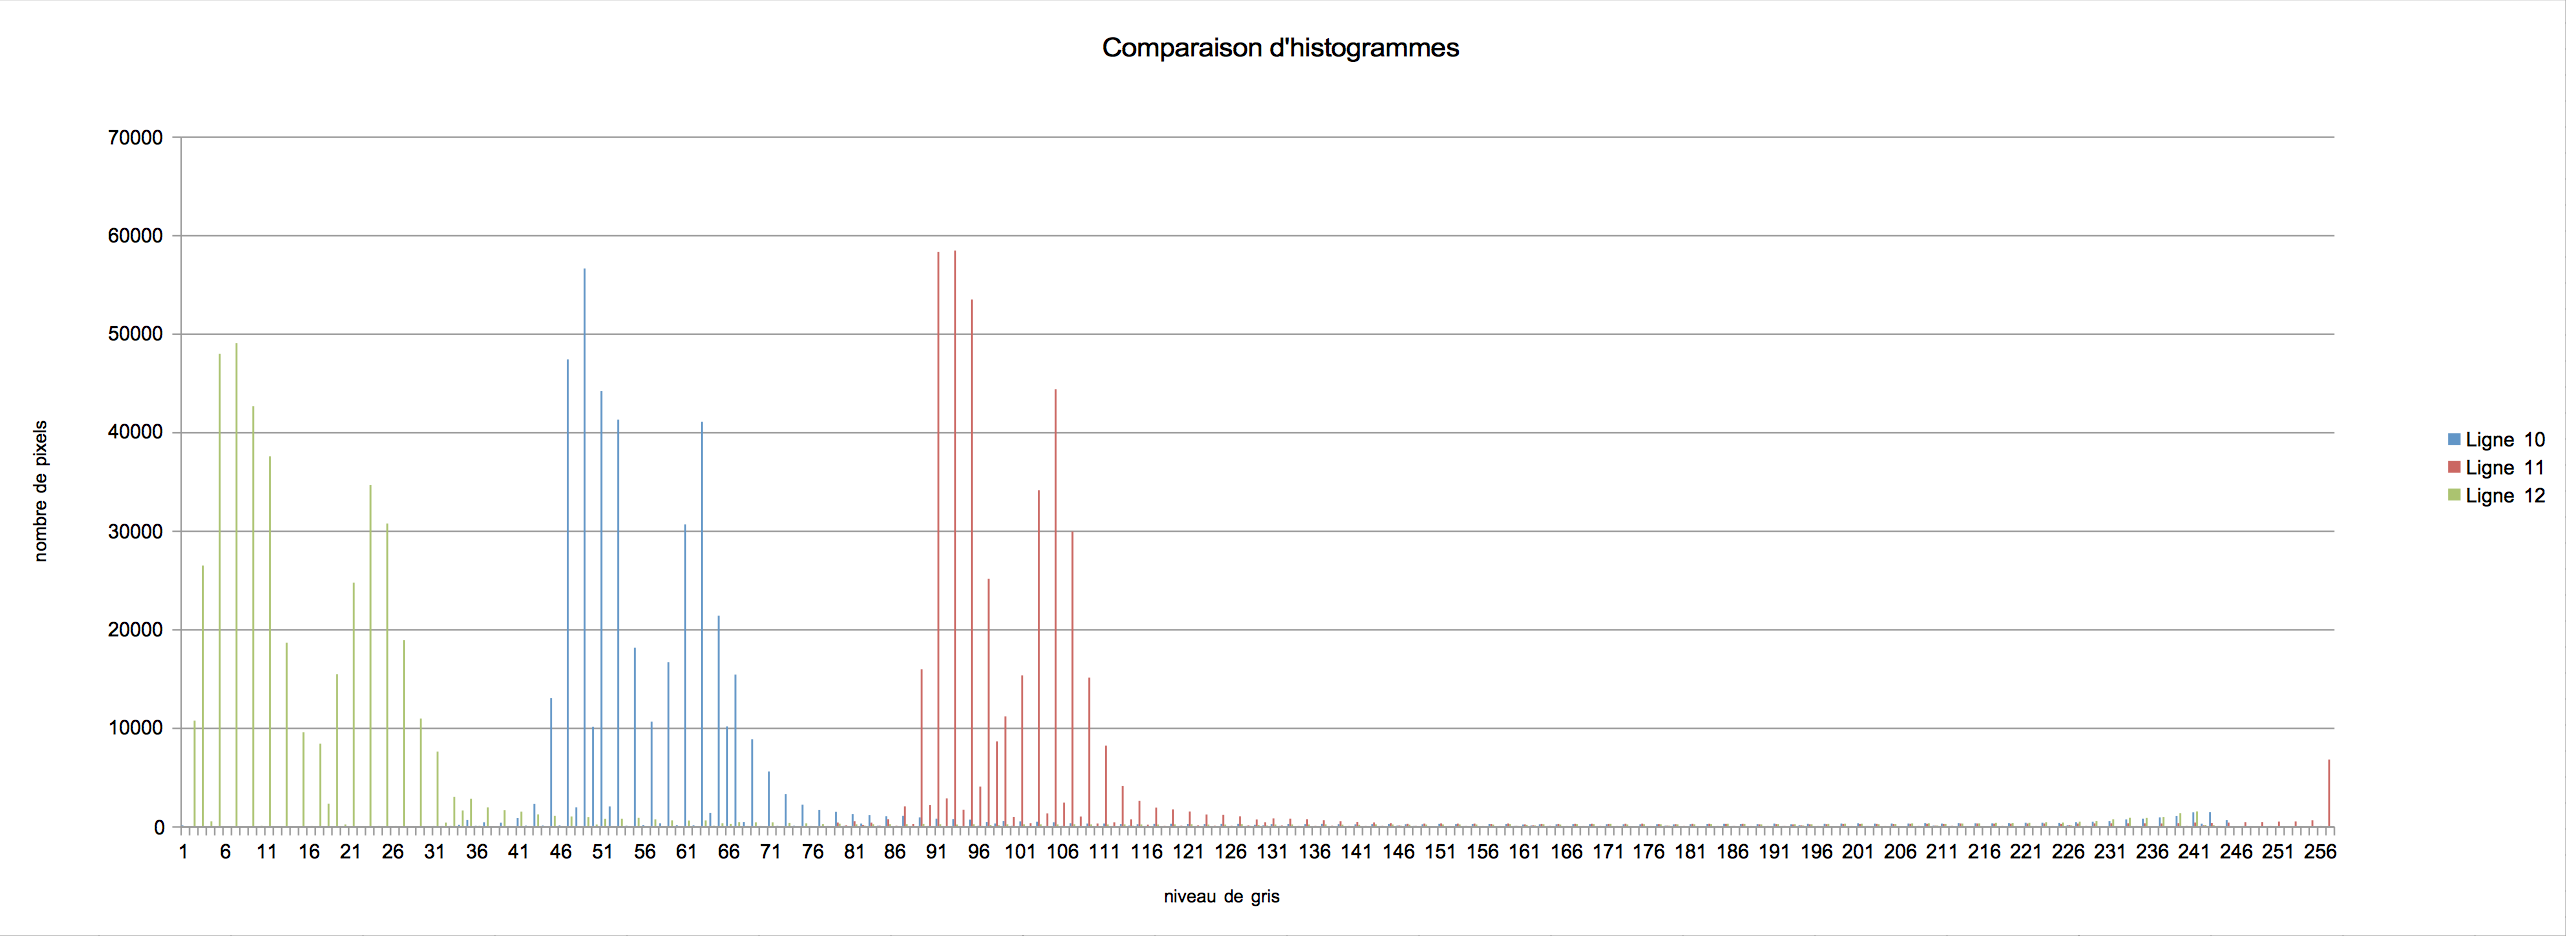
\includegraphics[width=15cm]{images/histogrammes1.png}
\caption{Histogrammes de Connect Ok L D}
\end{figure}

\begin{table}[!h]
	\begin{center}
		\begin{tabular}{|c|c|c|c|}
		   \hline
		   & Connect_D & Connect_OK & Connect_L \\
		   \hline
		   Les broches & [195,240]& [200,245] & [225,256]\\
		   \hline
		   Partie foncée & [0,76] & [30,116] & [76,161]\\
		   \hline
		\end{tabular}
	\end{center}
	\caption{Comparaisons : plage niveaux de gris}
\end{table}

\newpage
Sur les même images, nous avons également pris le temps de réaliser des comparaisons de profils de lignes. Le code couleur est le même
que pour les histogrammes. Nous avons pris soin d'augmenter le nombre d'échantillons pris pour les profils à 256 chacun. Chaque pic 
correspond à une broche. Le fait que les transitions fond/broche ne soient pas nettent est explicable soit par le fait que le nombre
d'échantillon (256 soit le maximum que l'on peut réaliser d'un point de vue technique ici) est insufisant soit par le fait que la résolution
du capteur qui a pris cette image n'est pas assez élevée.

\begin{figure}[!h]
\centering
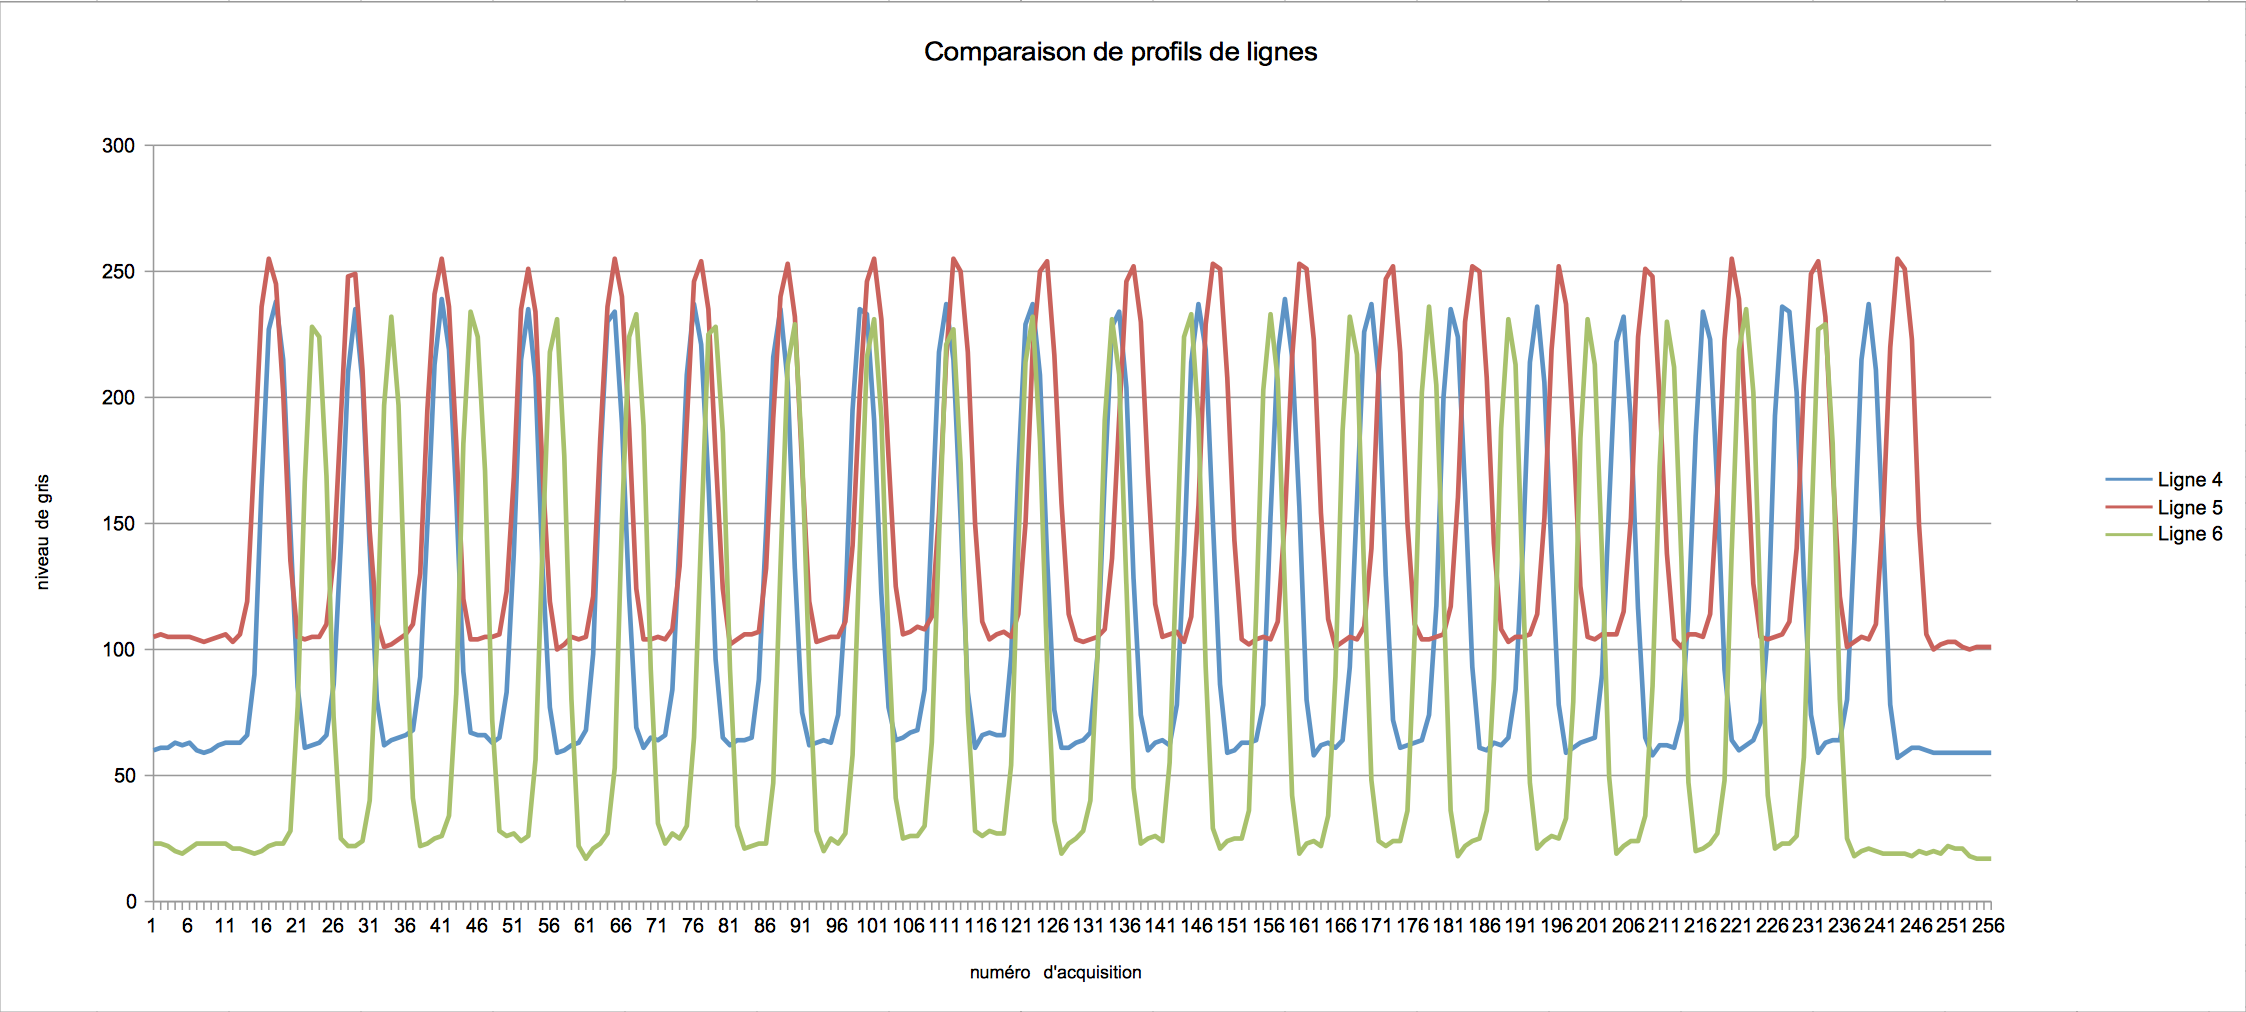
\includegraphics[width=15cm]{images/profildeligne1.png}
\caption{Profils de ligne de Connect Ok L D}
\end{figure}

\newpage
Maintenant, concentrons nous sur l'image PNCN256. Nous avons dans un premier temps réalisé l'histogramme de celle-ci. Nous observons que 
la dynamique de cette image s'étant du niveau de gris 0 au niveau de gris 200 environ. Il est difficile avec cet histogramme de séparer
les différents objets du fond. D'autant plus que, après réalisation du profil de ligne du allant du coin haut gauche au coin bas droite de l'image, on peut remarquer un problème 
d'éclairage de la scène. En effet, on a des niveaux de gris élevé du côté du coin haut gauche et des niveaux de gris plus faibles du côté 
du coin bas droite. Cela met en évidence un éclaire non homogène venant du coin haut gauche de l'image de la scène. 
  

\begin{figure}[!h]
\centering
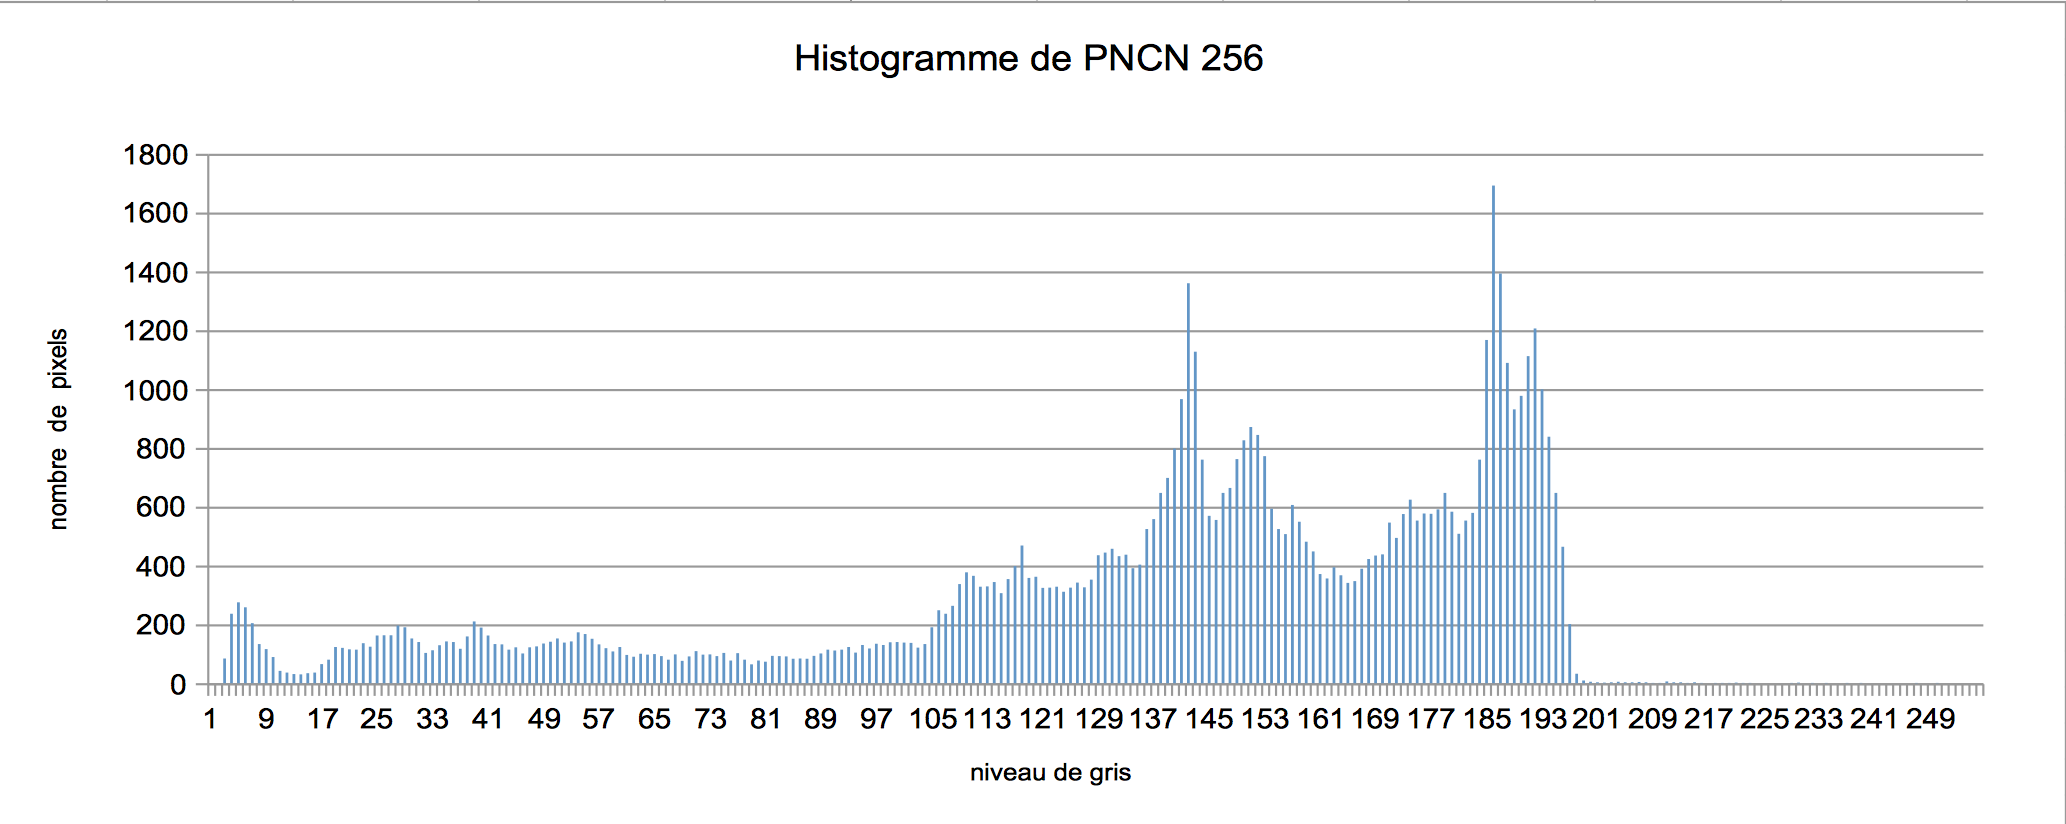
\includegraphics[width=15cm]{images/histogramme2.png}
\caption{Histogramme de PNCN 256}
\end{figure}

\begin{figure}[!h]
\centering
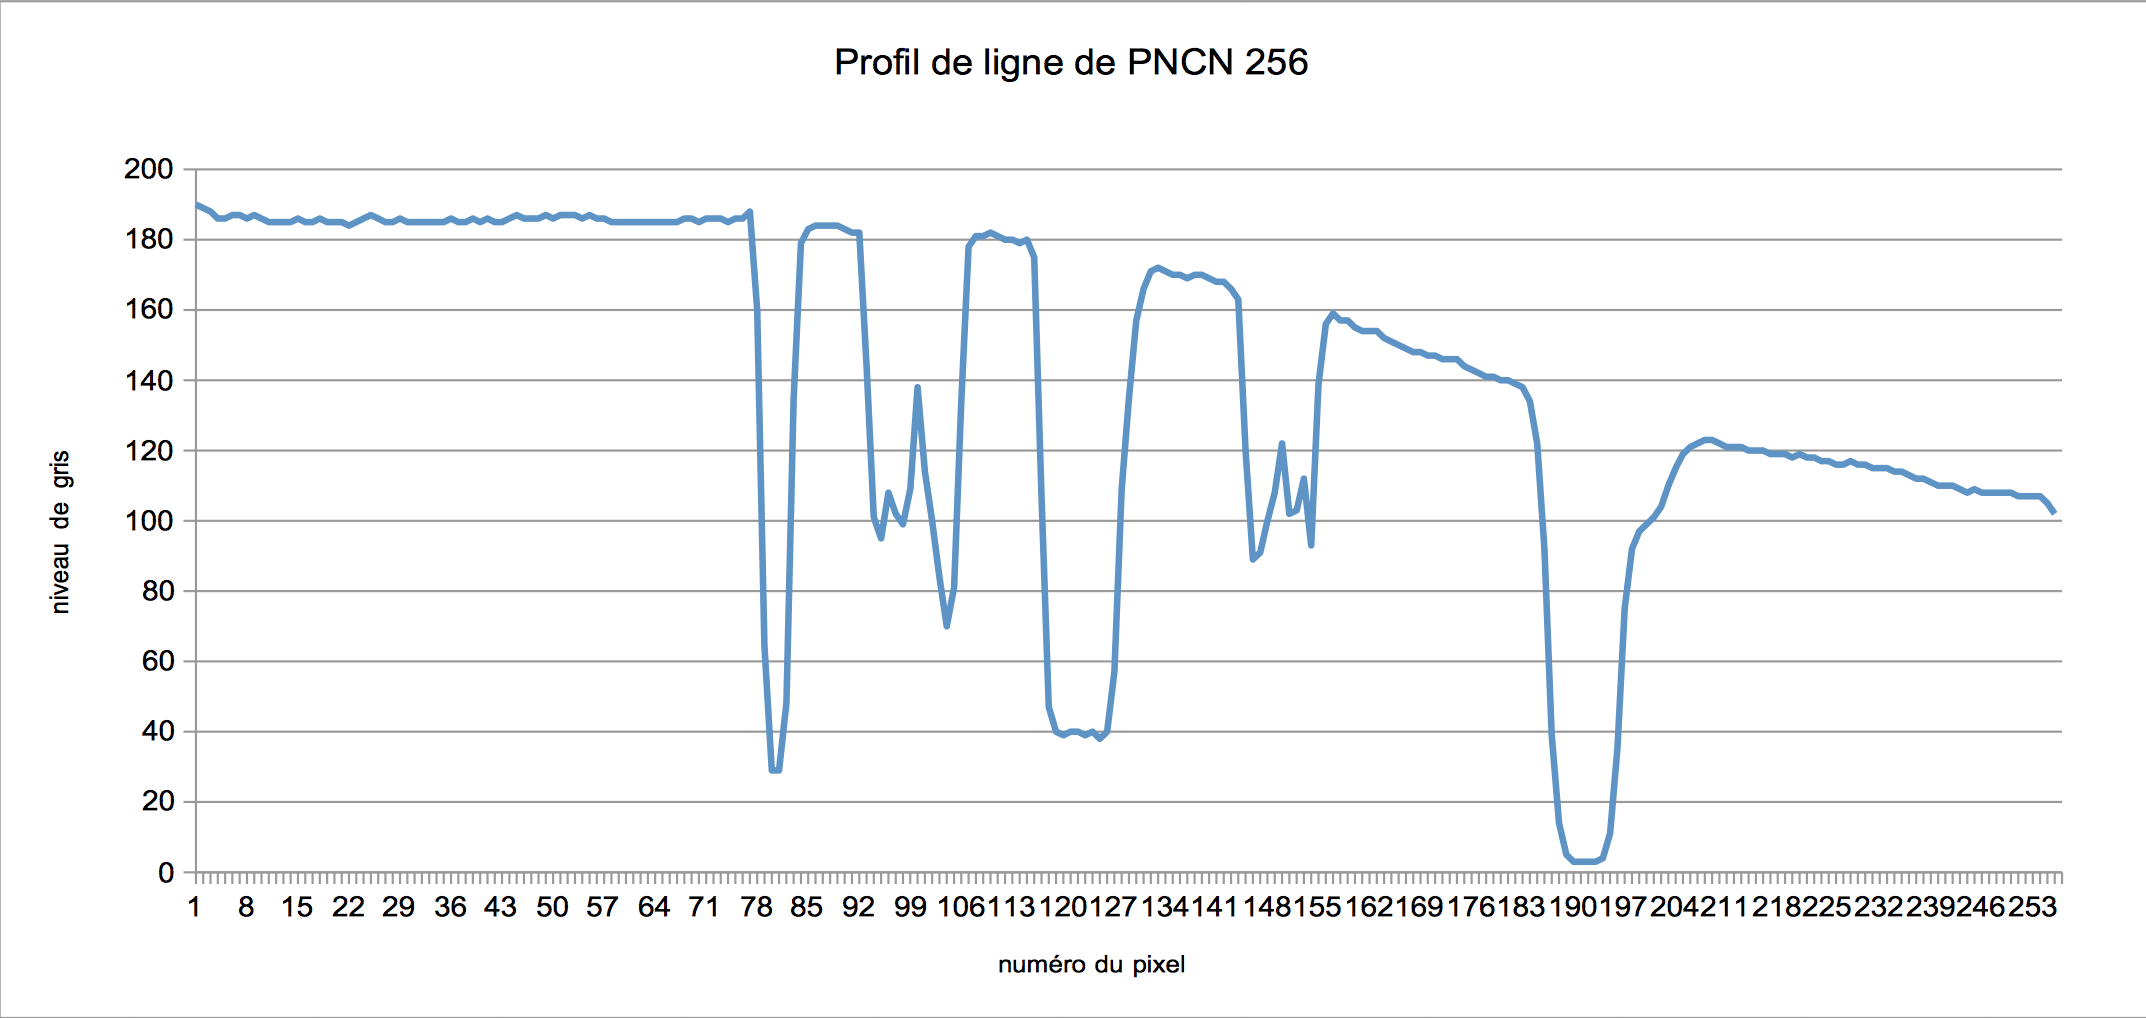
\includegraphics[height=5cm,width=15cm]{images/profildeligne2.png}
\caption{Profil de ligne de PNCN 256}
\end{figure}

\newpage
\section{Traitements d'amélioration par LUT}
\addcontentsline{toc}{section}{Traitements d'amélioration par LUT}

Le premier objectif qui nous a été posé dans cette section, est de réaliser deux LUT. 
En effet, on désire réajuster numériquement les problèmes d'éclairage des images 
Connect_L et Connect_D dont nous nous sommes rendu-compte précédemment. 
Pour ce faire, on a dû réajuster les encadrements de niveaux de gris observés dans la
première section. La figure suivante nous montre les LUTs appliquées respectivement à 
l'image Connect_L et Connect_D. Celles-ci ne sont pas très précises, compte-tenu du 
fait qu'elles ont été faites à main levée.  

\begin{figure}[H]
\centering
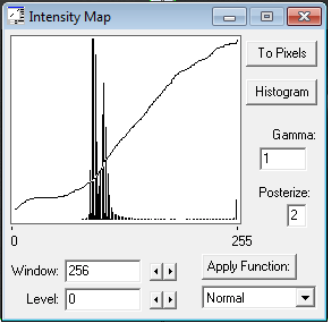
\includegraphics[height=5cm,width=5cm]{images/lut1.png} \hfill
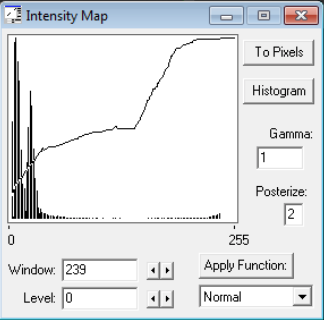
\includegraphics[height=5cm,width=5cm]{images/lut2.png}
\caption{LUTs appliquées respectivement à Connect_L et Connect_D}
\end{figure}

Le deuxième objectif a été de réutiliser l'outil Threshold afin d'effectuer un seuillage
qui nous permettrait de ne faire apparaitre que les broches. Nous pouvons constater d'après la figure
suivante que placer le seuil au niveau de gris 131 est suffisant. Ainsi si nous réalisions une LUT
où on aurait 0 en ordonnée du niveau de gris 0 au niveau de gris 131, et, où on aurait 255 en 
ordonnée du niveau de gris 131 au niveau de gris 255, on ne verrait que les broches en blanc sur
un fond noir.  

\begin{figure}[H]
\centering
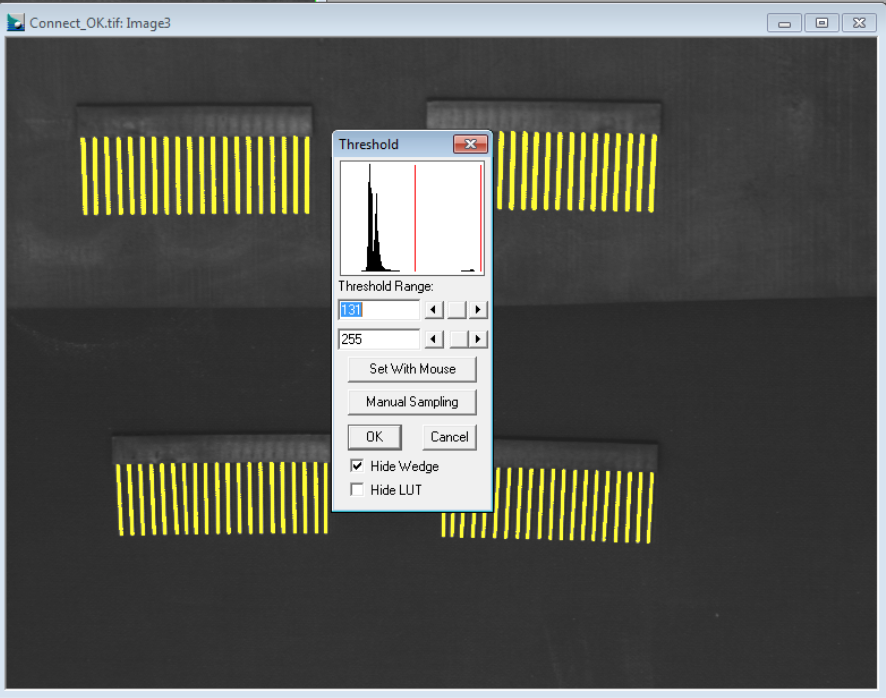
\includegraphics[height=5cm,width=7.5cm]{images/threshold1.png}
\caption{Seuillage grâce à l'outil Threshold}
\end{figure}

\newpage
Il est difficile manuellement de définir un seuil exacte pour ne récupérer que les broches.
En effet, l'histogrammes ne présente pas un pic bien définit représentant le niveau de gris 
des broches. Un trop grand nombre de niveaux de gris représente en fait la transition entre
les broches et le reste de l'image. Le seuillage automatique proposé par l'outil nous donne 
les valeurs suivante : 

\begin{table}[H]
        \begin{center}
                \begin{tabular}{|c|c|c|}
                   \hline
                   & Seuil bas & Seuil haut \\
                   \hline
                   Manuel & 125 & 255\\
                   \hline
                   Automatique & 131 & 255\\
                   \hline
                \end{tabular}
        \end{center}
        \caption{Comparaisons : seuils de niveaux de gris}
\end{table} 

On constate néanmoins pour cet échantillon de données un faible écart du seuil bas.

\chapter{Deuxième partie}
\addcontentsline{toc}{chapter}{Deuxième partie}

\begin{center}
\large{
\textbf{Traitements aux environs du pixel.}}
\end{center}

\section{Passe bas}
\addcontentsline{toc}{section}{Passe bas}

Pour ce début de deuxième partie, nous devons mettre en évidence les différences entre divers applications de filtres passe-bas.
On voit tout d'abord qu'un filtre gaussien avec un masque 3x3 garde l'image plus nette que le filtre gaussian 5x5. Ce résultat semble logique
puisqu'en effet, un masque 5x5 prend en compte beaucoup plus de pixel qu'un masque 3x3.

De plus, nous remarquons qu'un filtre médian qui est en fait une opération non linéaire contrairement au filtre gaussien, réduit beaucoup plus le bruit
dans le cas de l'image MEDIAN.tif

Voici les résultats obtenus. 

\begin{figure}[!h]
\centering
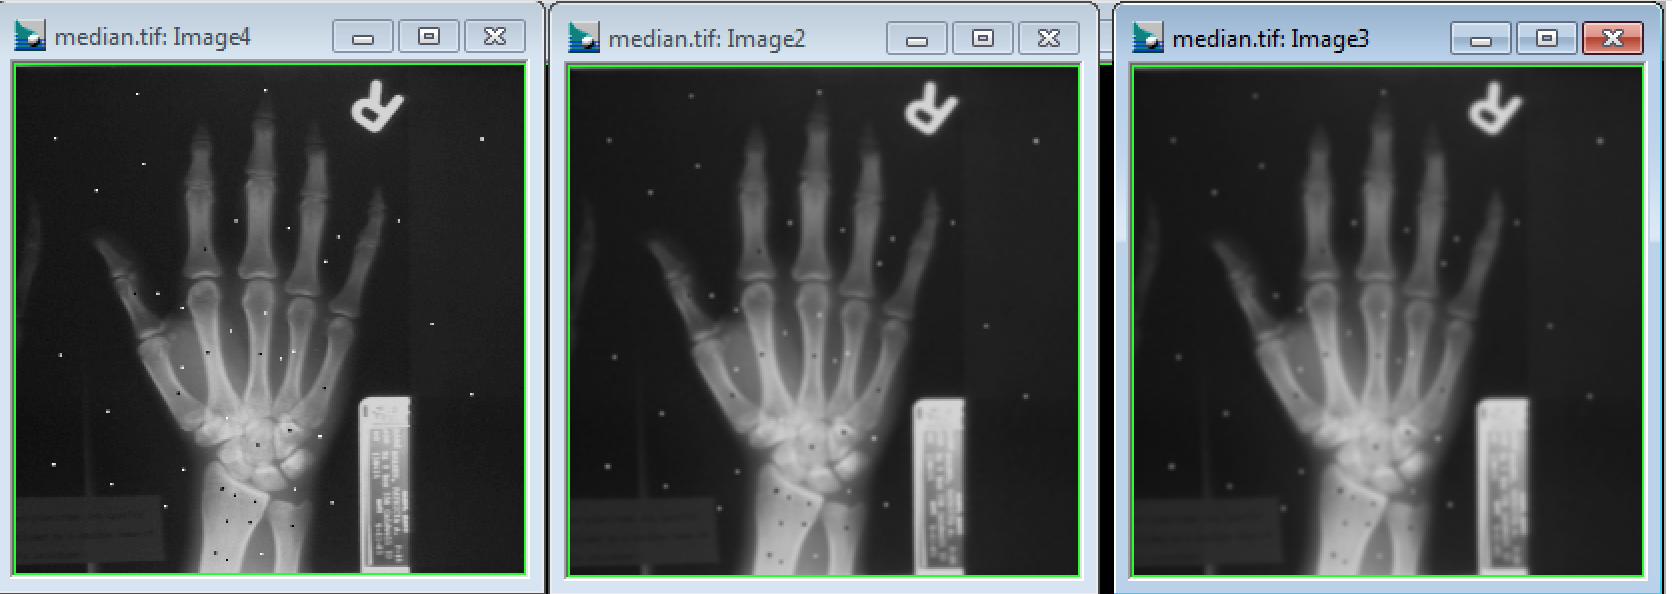
\includegraphics[height=5cm,width=15cm]{images/gaussian.png}
\caption{Comparaison image Median.tif non filtrée, filtrée Gaussian 3x3, filtrée Gaussian 5x5}
\end{figure}

\newpage
\begin{figure}[!h]
\centering
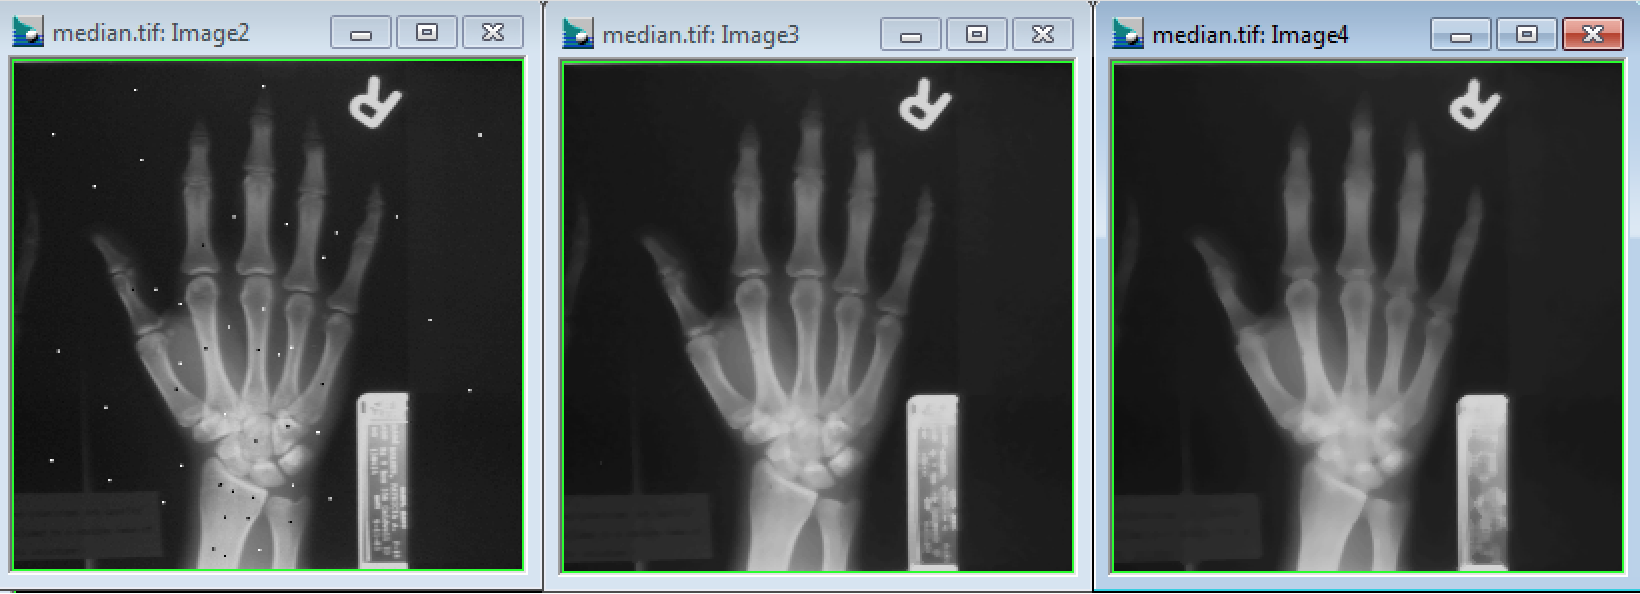
\includegraphics[height=5cm,width=15cm]{images/median.png}
\caption{Comparaison image Median.tif non filtrée, filtrée Median 3x3, filtrée Median 5x5}
\end{figure}

Dans une deuxième partie, on se propose, toujours pour la même image de réaliser d'appliquer un filtre passe-bas
grâce à la Transformée de Fourier, notion de traitement du signal adaptée ici au traitement d'une image. 
On voit donc sur la figure suivante la représentation graphique des fréquences de l'image Median.tif 

\begin{figure}[!h]
\centering
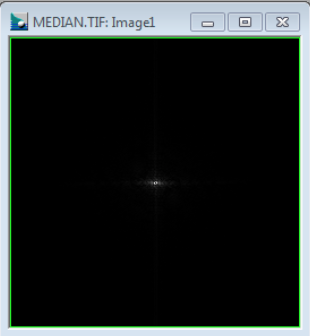
\includegraphics[height=5cm,width=5cm]{images/tfmedian.png}
\caption{Représentation de la transformée de Fourier appliquée à l'image Median.tif}
\end{figure}

Ensuite, pour réaliser le filtre, il faut réaliser avec le logiciel une zone d'application que l'on concervera. 
On doit en effet, laisser les basses fréquences et supprimer les hautes fréquence à l'aide de la commande "zeros outside" d'Optimas.
De cette manière, le bruit impulsionnelle (représenté en transformée de Fourier par les hautes fréquences) sera supprimé.

\newpage
Voici un apperçu des fréquences gardées. 

\begin{figure}[!h]
\centering
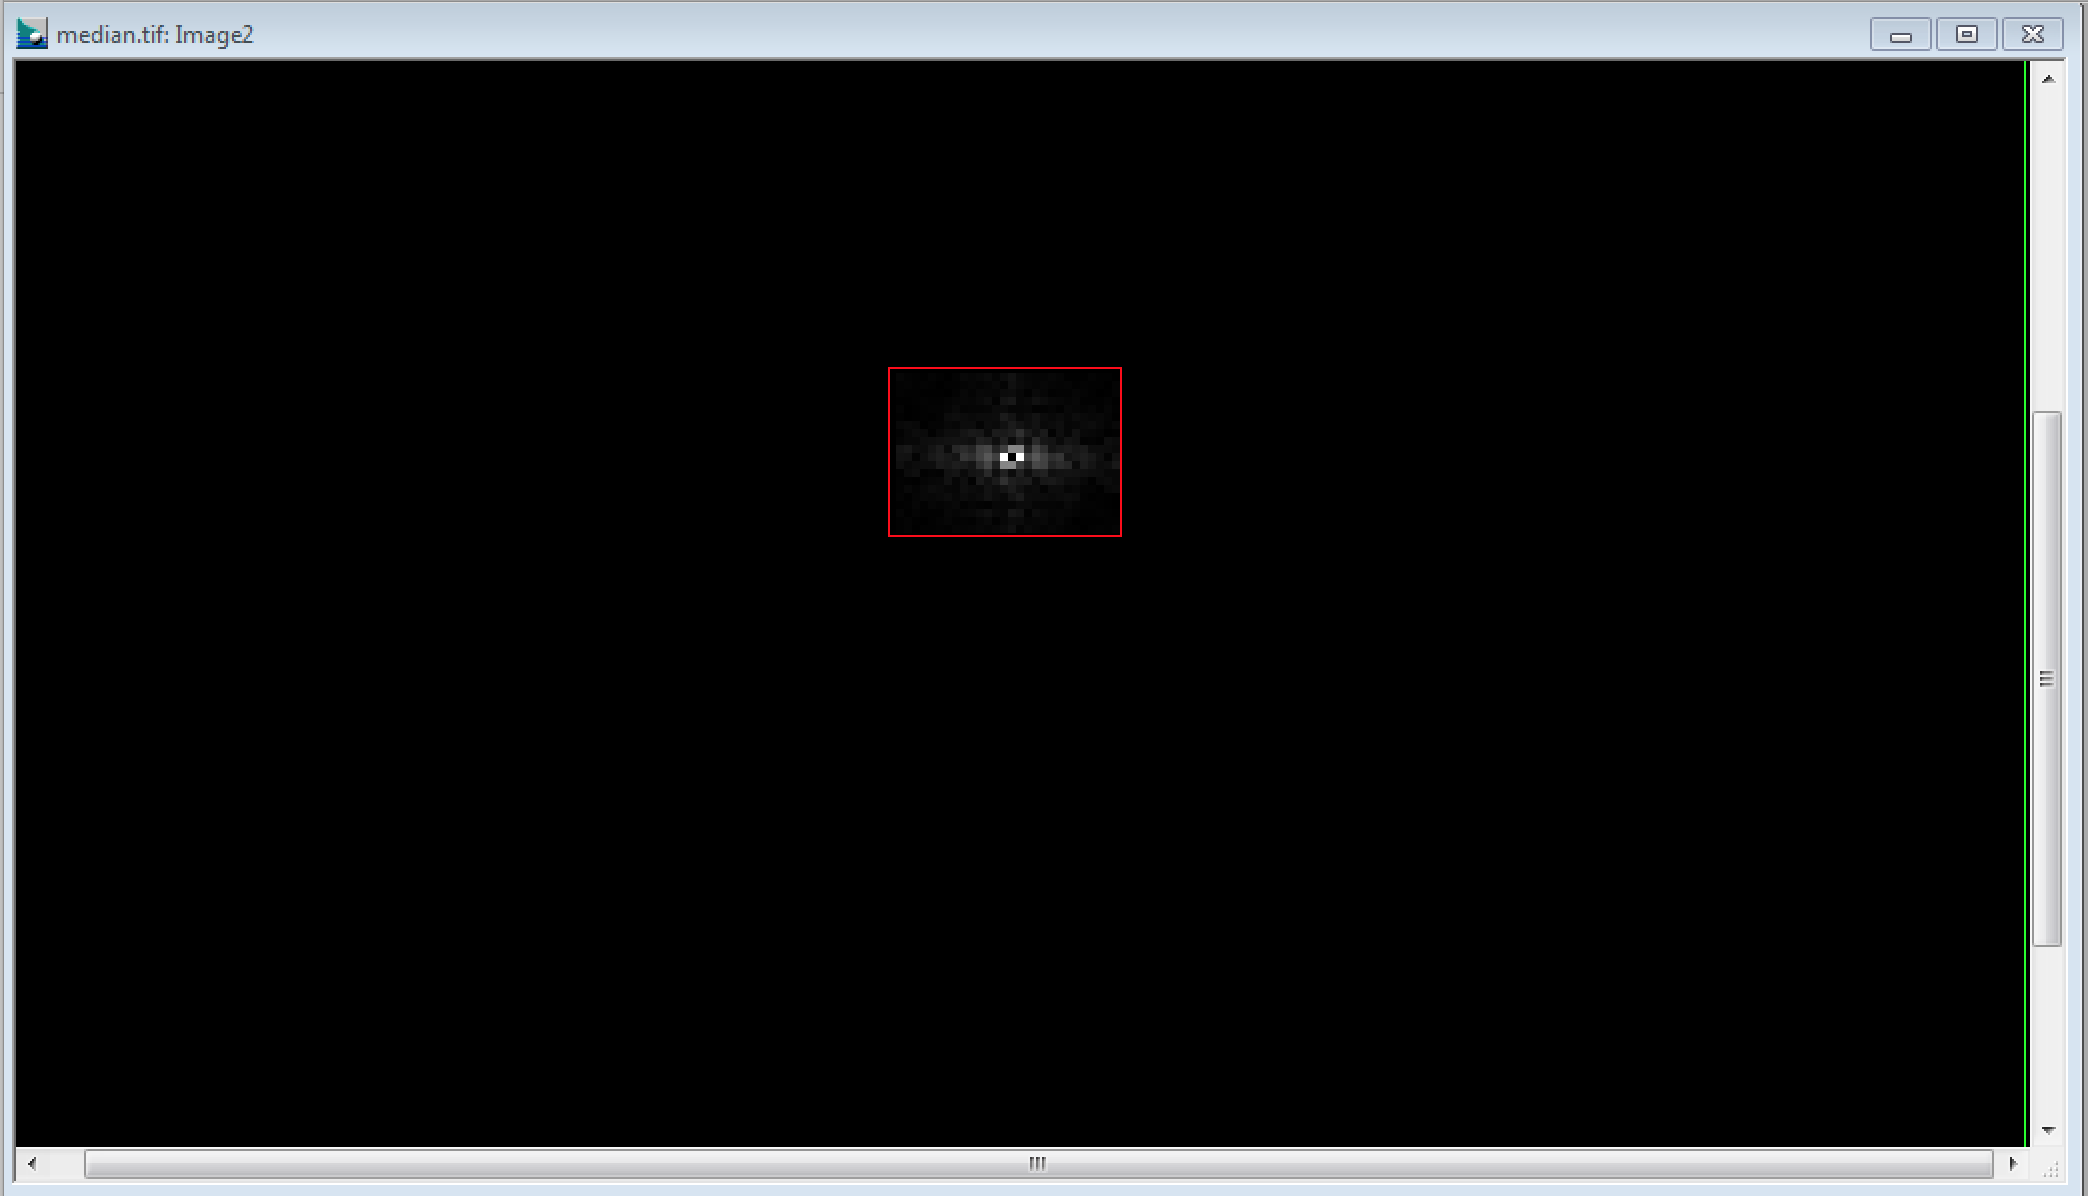
\includegraphics[height=5cm,width=5cm]{images/tfmediancut.png}
\caption{Représentation de la transformée de Fourier appliquée à l'image Median.tif découpée}
\end{figure}

Néanmoins, lorsque nous avons réalisé le transformée inverse, nous avons constaté que le bruit n'avait pas été supprimé correctement. 

\begin{figure}[!h]
\centering
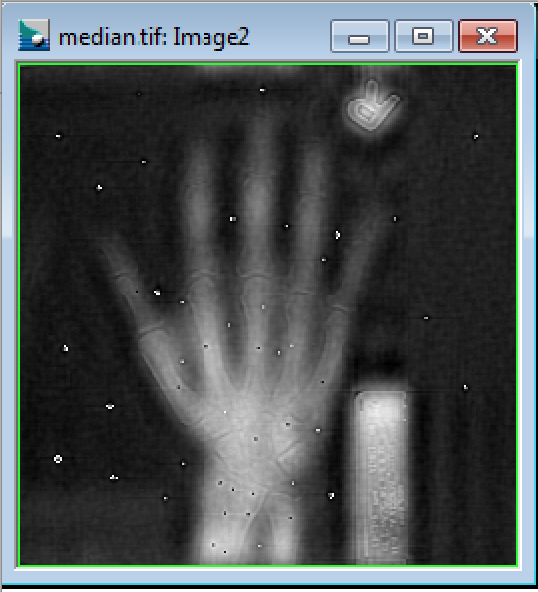
\includegraphics[height=5cm,width=5cm]{images/mediancut.png}
\caption{Filtrage avec la méthode décrite}
\end{figure}

\newpage


\section{Réhaussement de contours}
\addcontentsline{toc}{section}{Réhaussement de contours}

Nous voulons maintenant utiliser des filtres de réhaussement de contours pour mettre en évidence l'un phénomènes liés au système optique humain, 
le phénomène de Mach. On dit que le système optique humain a un comportement intégrateur.
Nous pouvons remarquer que les différents filtres amplifient les lignes intermédiaires entre les différentes colonnes de niveau de gris.
Le sharpenlow et le sharpenmid n'amplifient pas beaucoup ce phénomène contrairement au sharpenhigh. 
Voici un apperçu. 

\begin{figure}[!h]
\centering
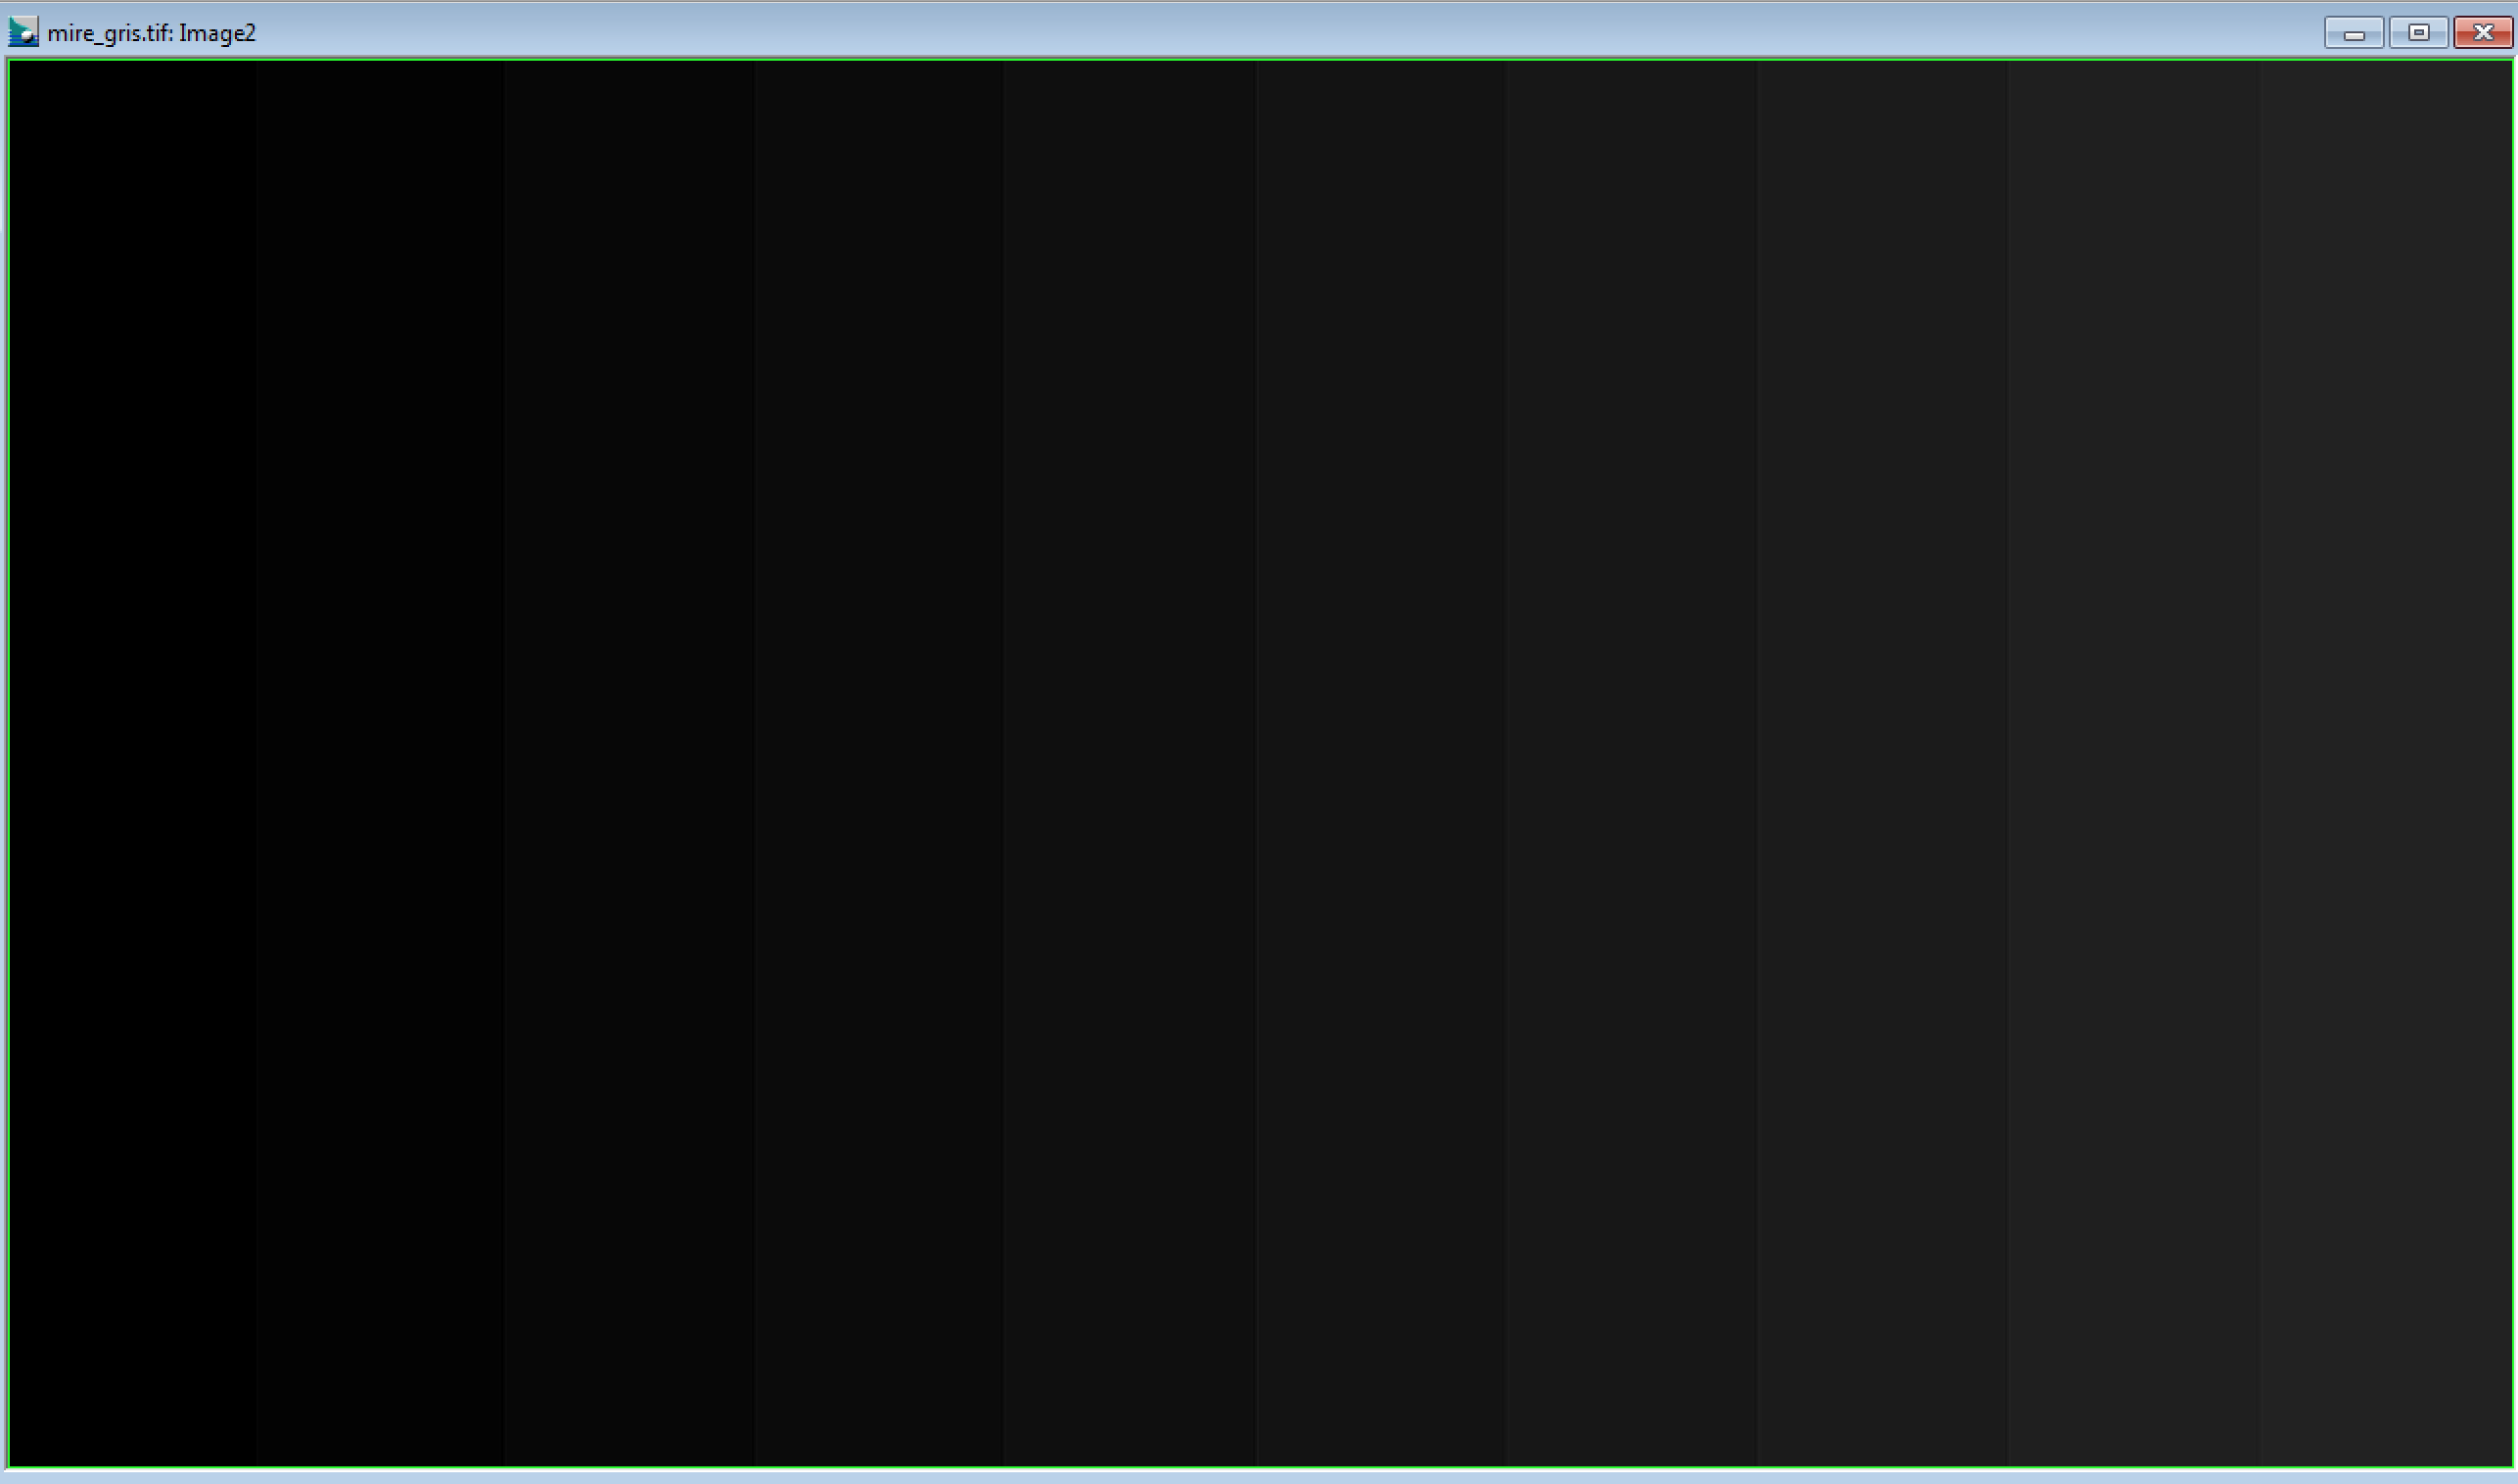
\includegraphics[height=5cm,width=15cm]{images/sharpenlow.png}
\caption{Utilisation de Sharpen Low mire_gris.tif}
\end{figure}

\begin{figure}[!h]
\centering
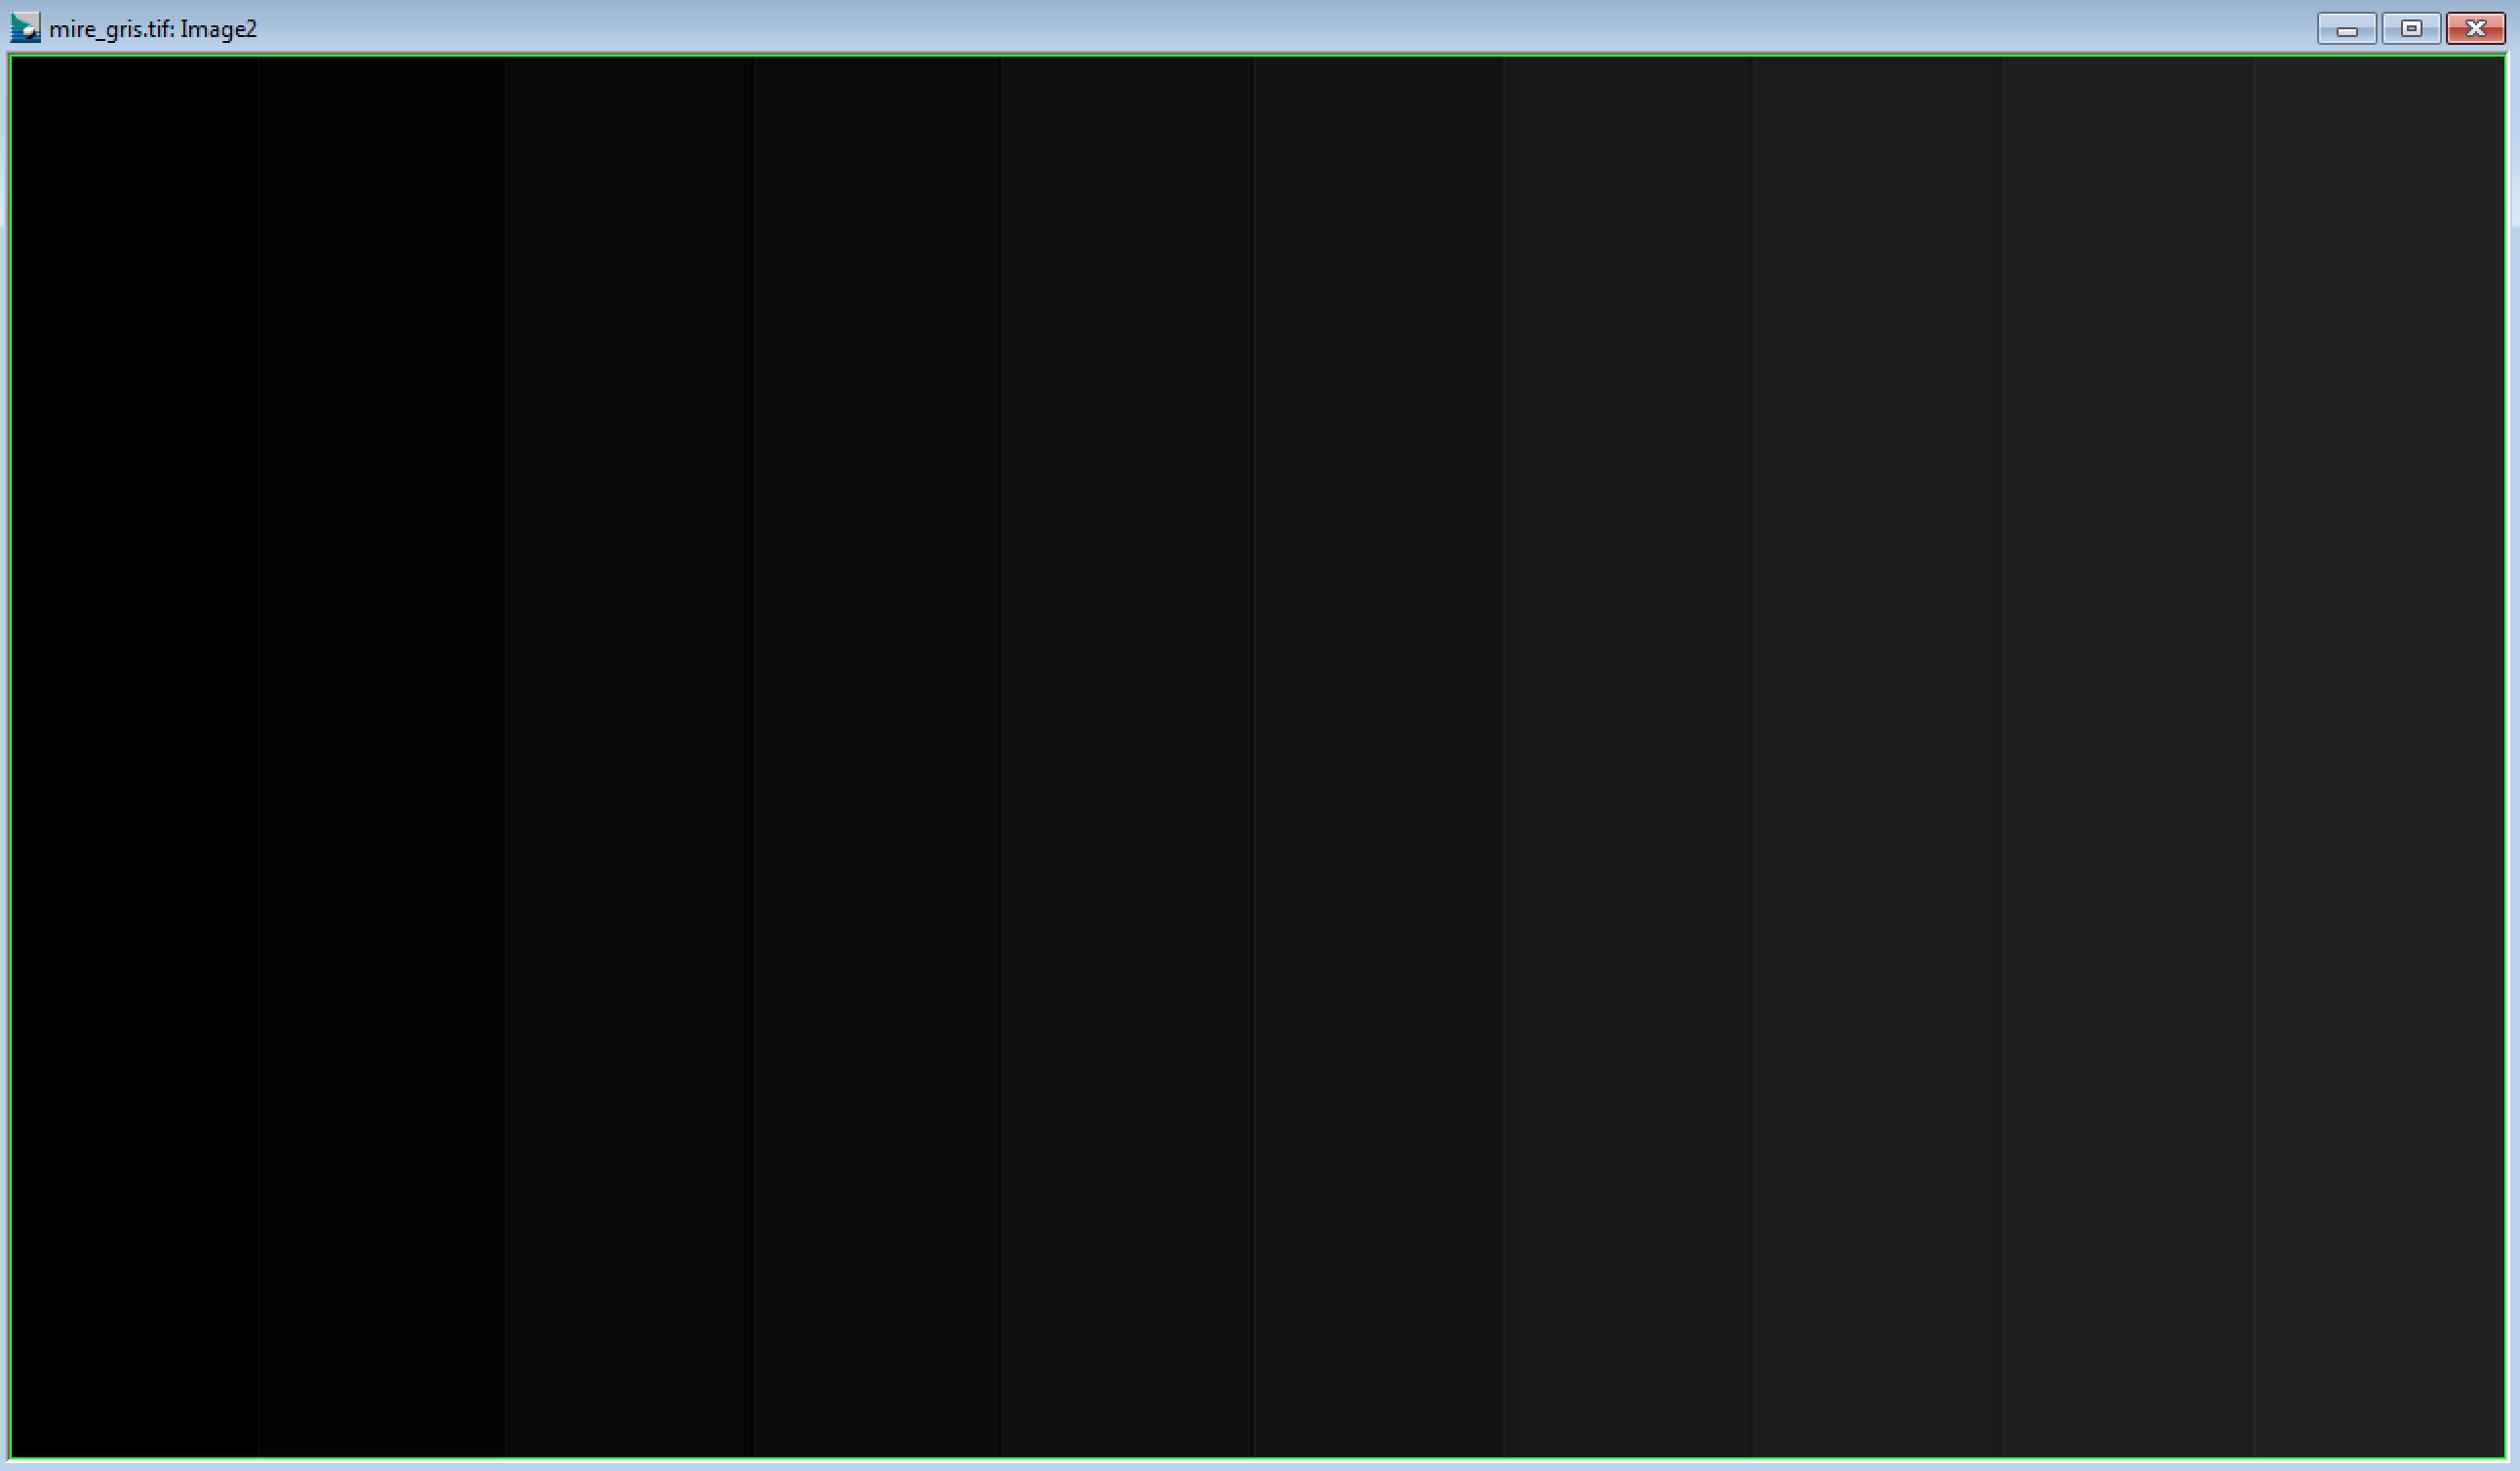
\includegraphics[height=5cm,width=15cm]{images/sharpenmid.png}     
\caption{Utilisation de Sharpen mid mire_gris.tif}
\end{figure}

\begin{figure}[!h]
\centering
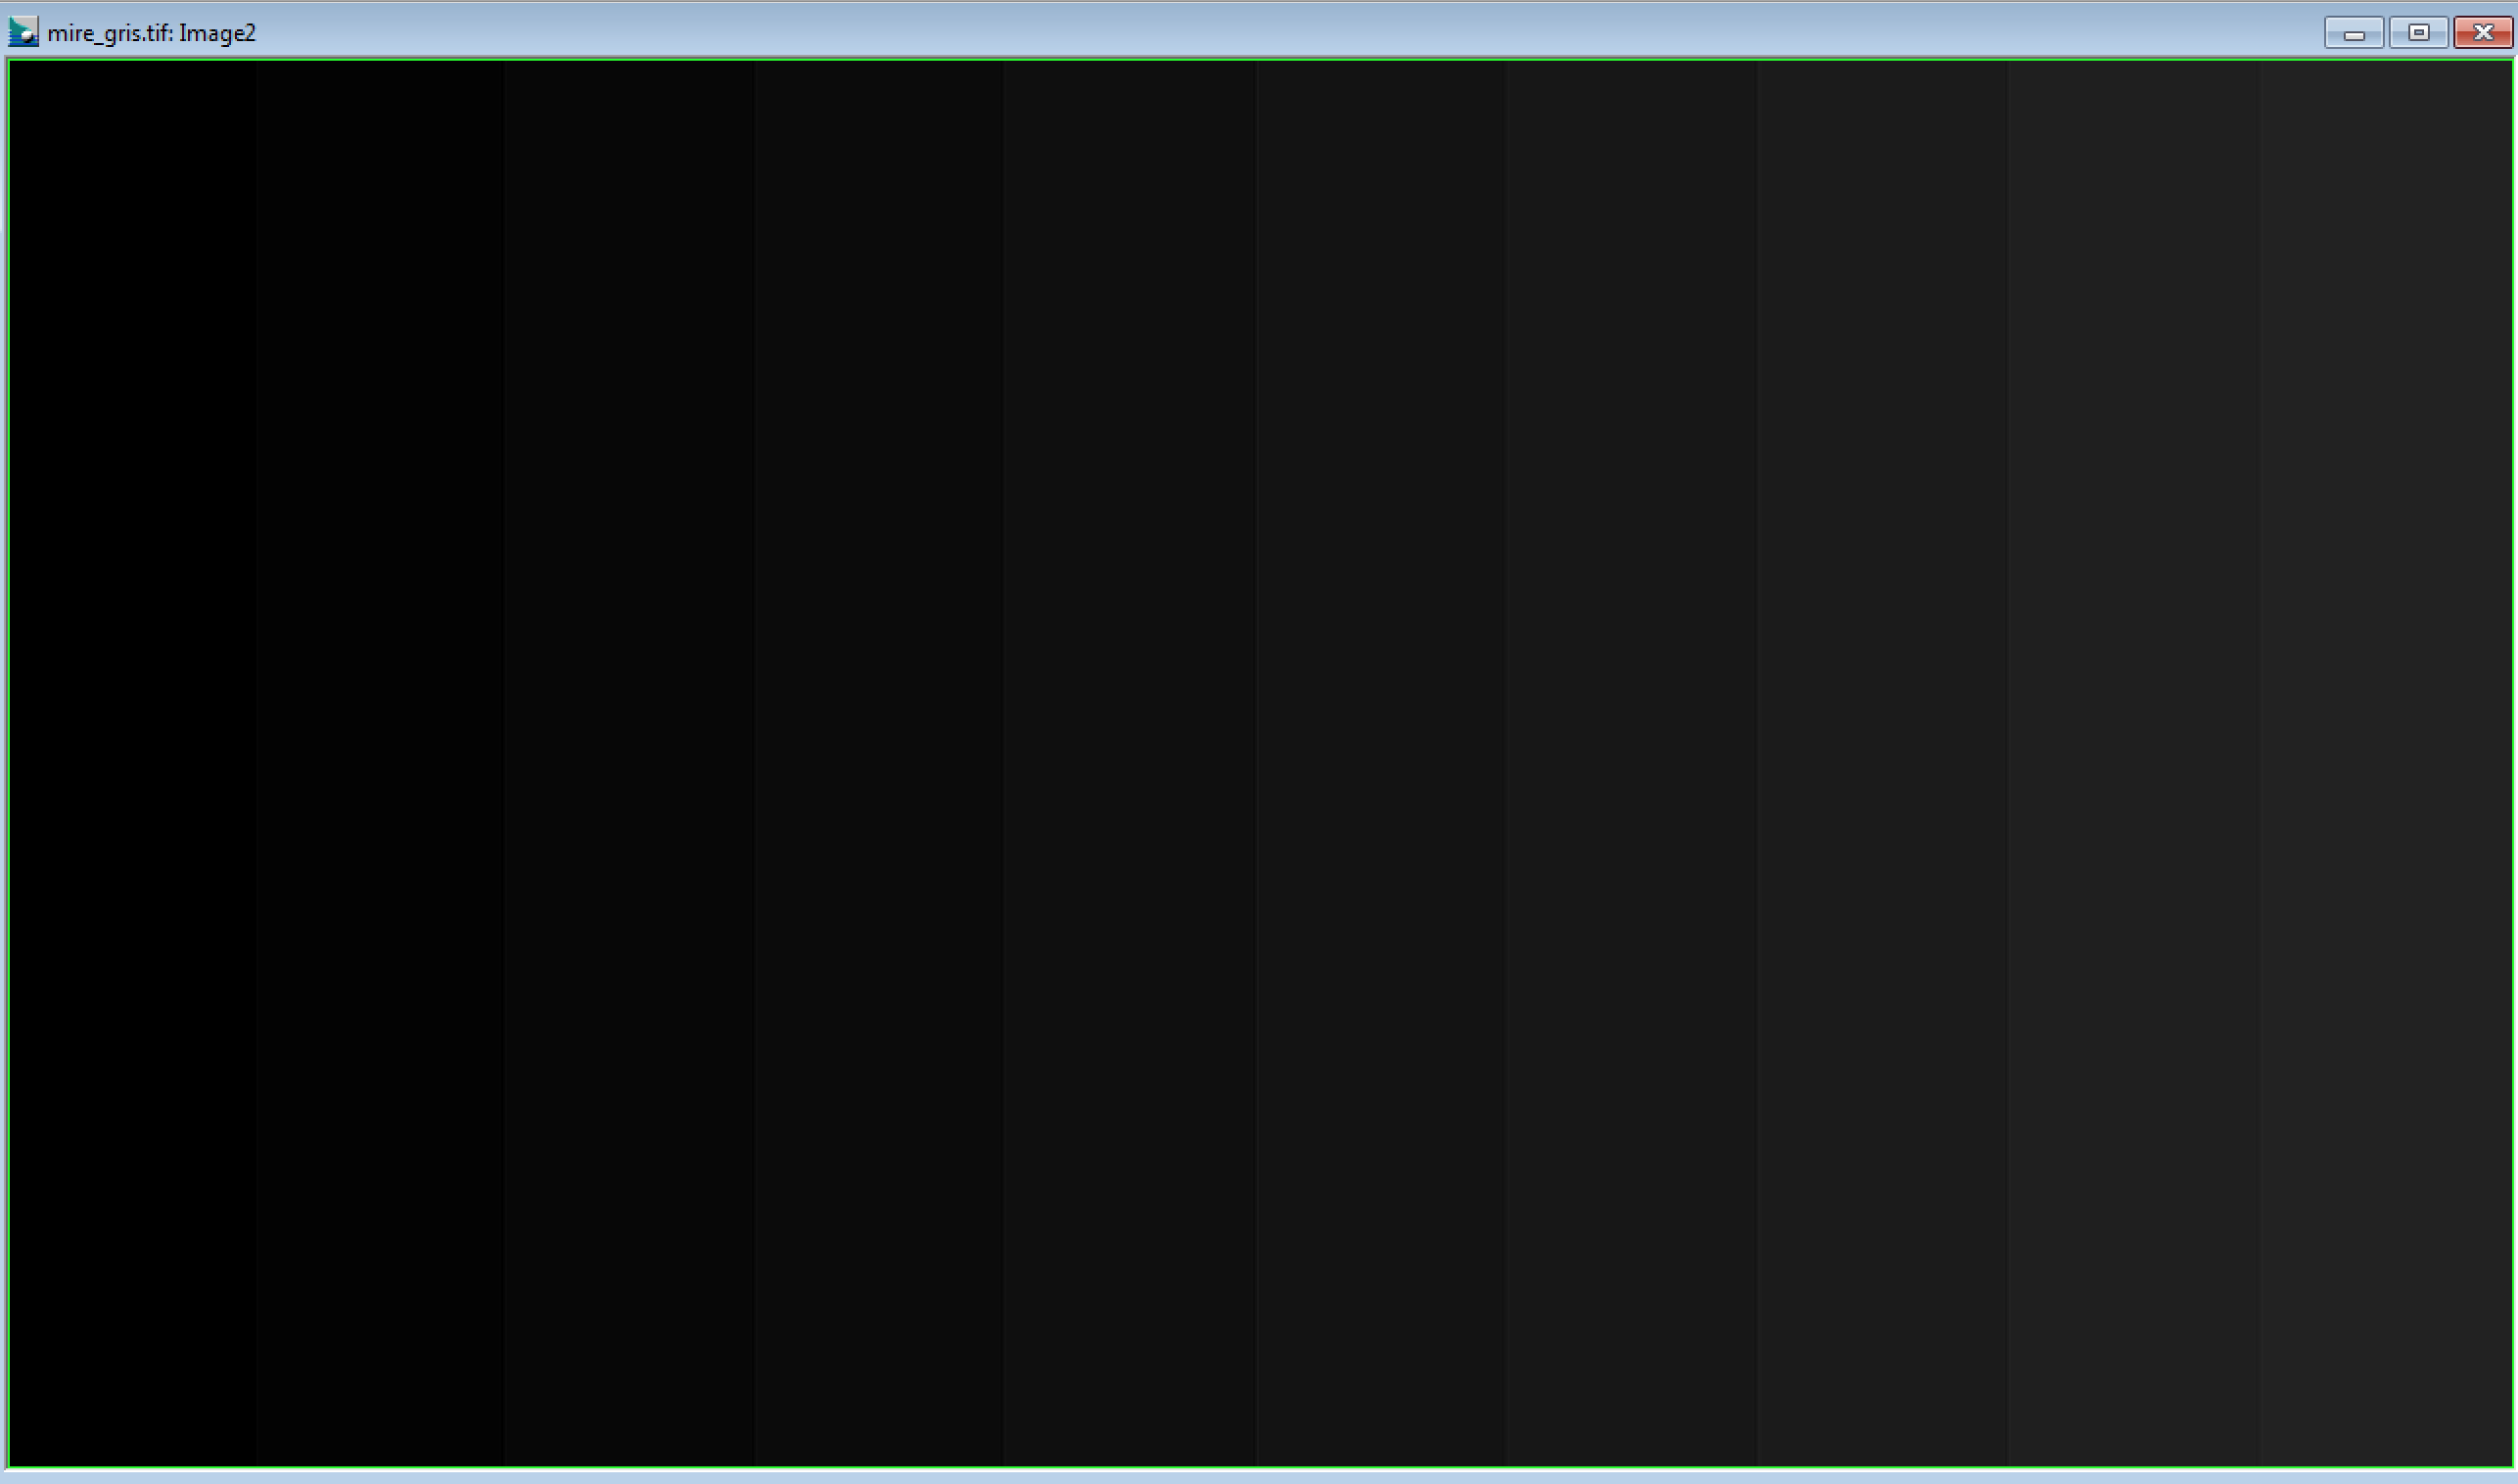
\includegraphics[height=5cm,width=15cm]{images/sharpenlow.png}     
\caption{Utilisation de Sharpen Low mire_gris.tif}
\end{figure}
  
\newpage
Pour mieux constater l'influence de ces différents filtres, nous avons choisi de tracer les profils de lignes suivant.

\begin{figure}[!h]
\centering
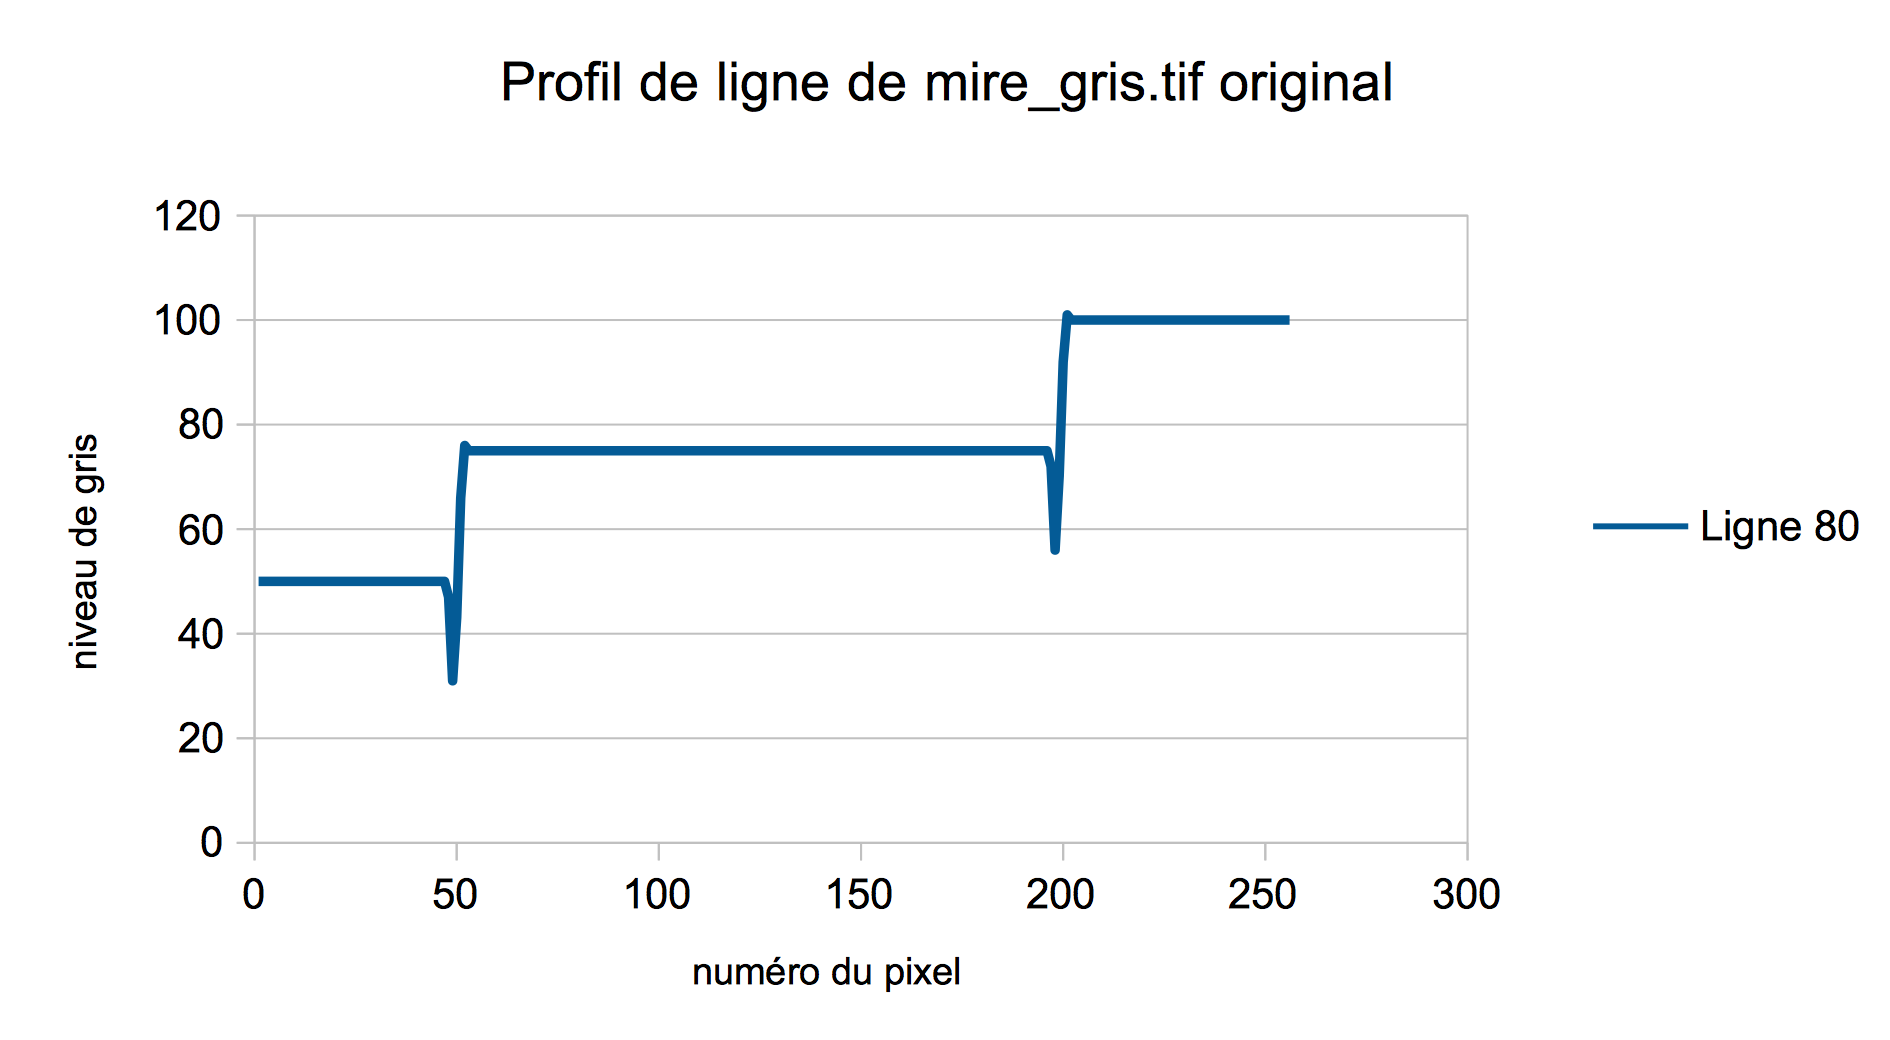
\includegraphics[height=7.5cm,width=15cm]{images/profillignemiregris.png}
\caption{Profil de ligne de l'image mire_gris.tif}
\end{figure}

\begin{figure}[!h]
\centering
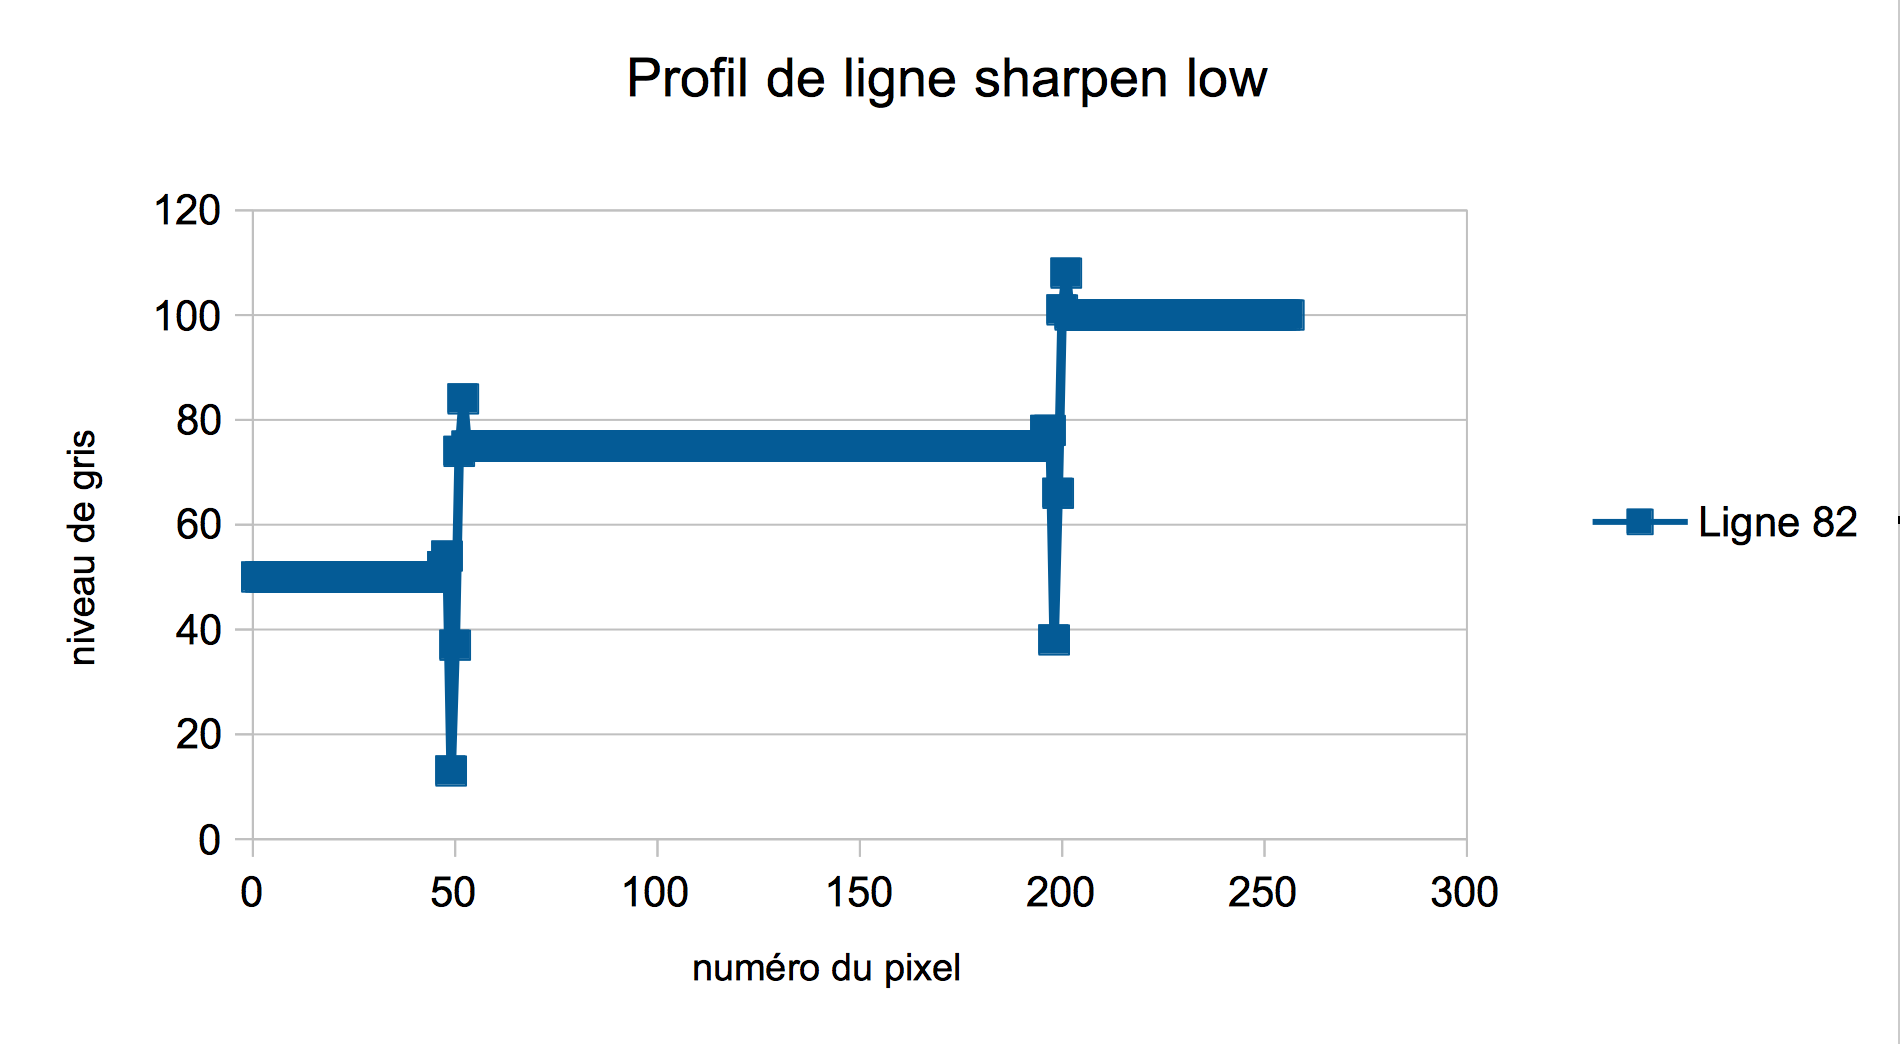
\includegraphics[height=7.5cm,width=15cm]{images/profillignesharpenlow.png}
\caption{Profil de ligne de l'image mire_gris.tif auquel on a appliqué un filtre sharpen low}
\end{figure}

\newpage
\begin{figure}[!h]
\centering
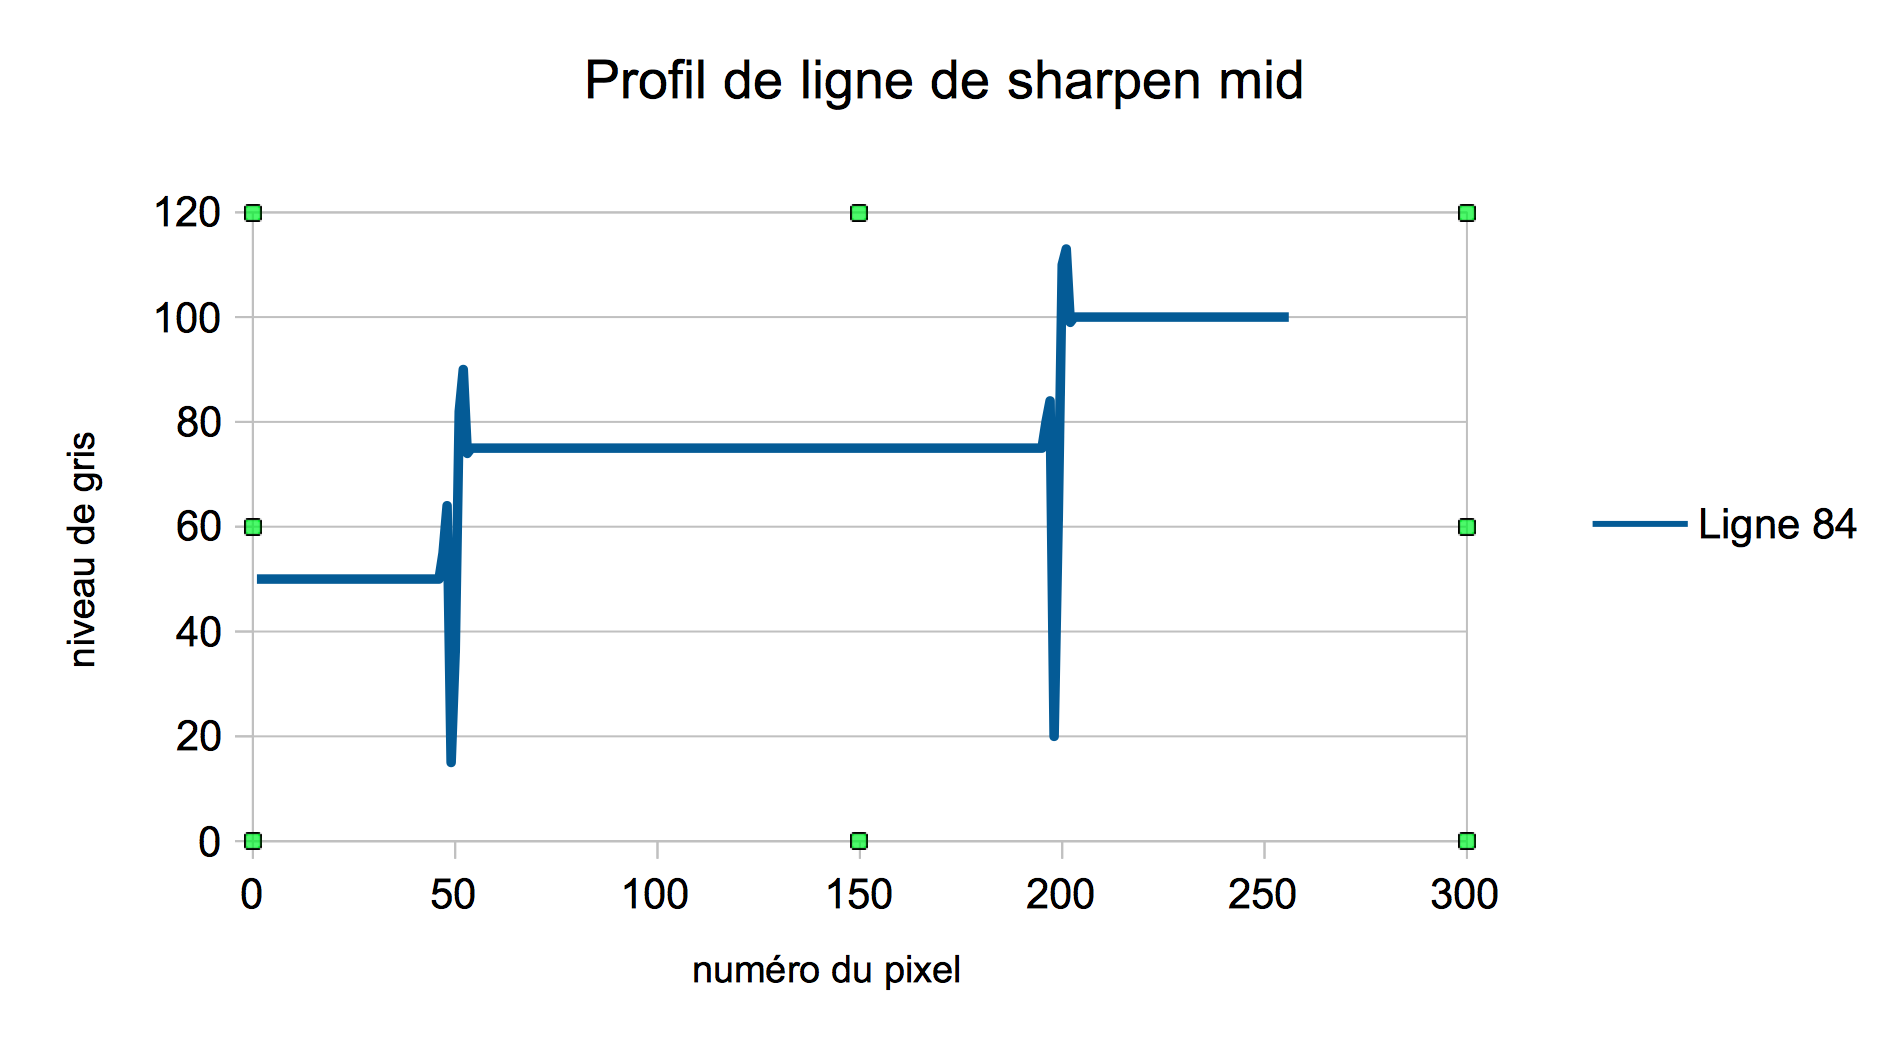
\includegraphics[height=7.5cm,width=15cm]{images/profillignesharpenmid.png}
\caption{Profil de ligne de l'image mire_gris.tif auquel on a appliqué un filtre sharpen mid}
\end{figure}

\begin{figure}[!h]
\centering
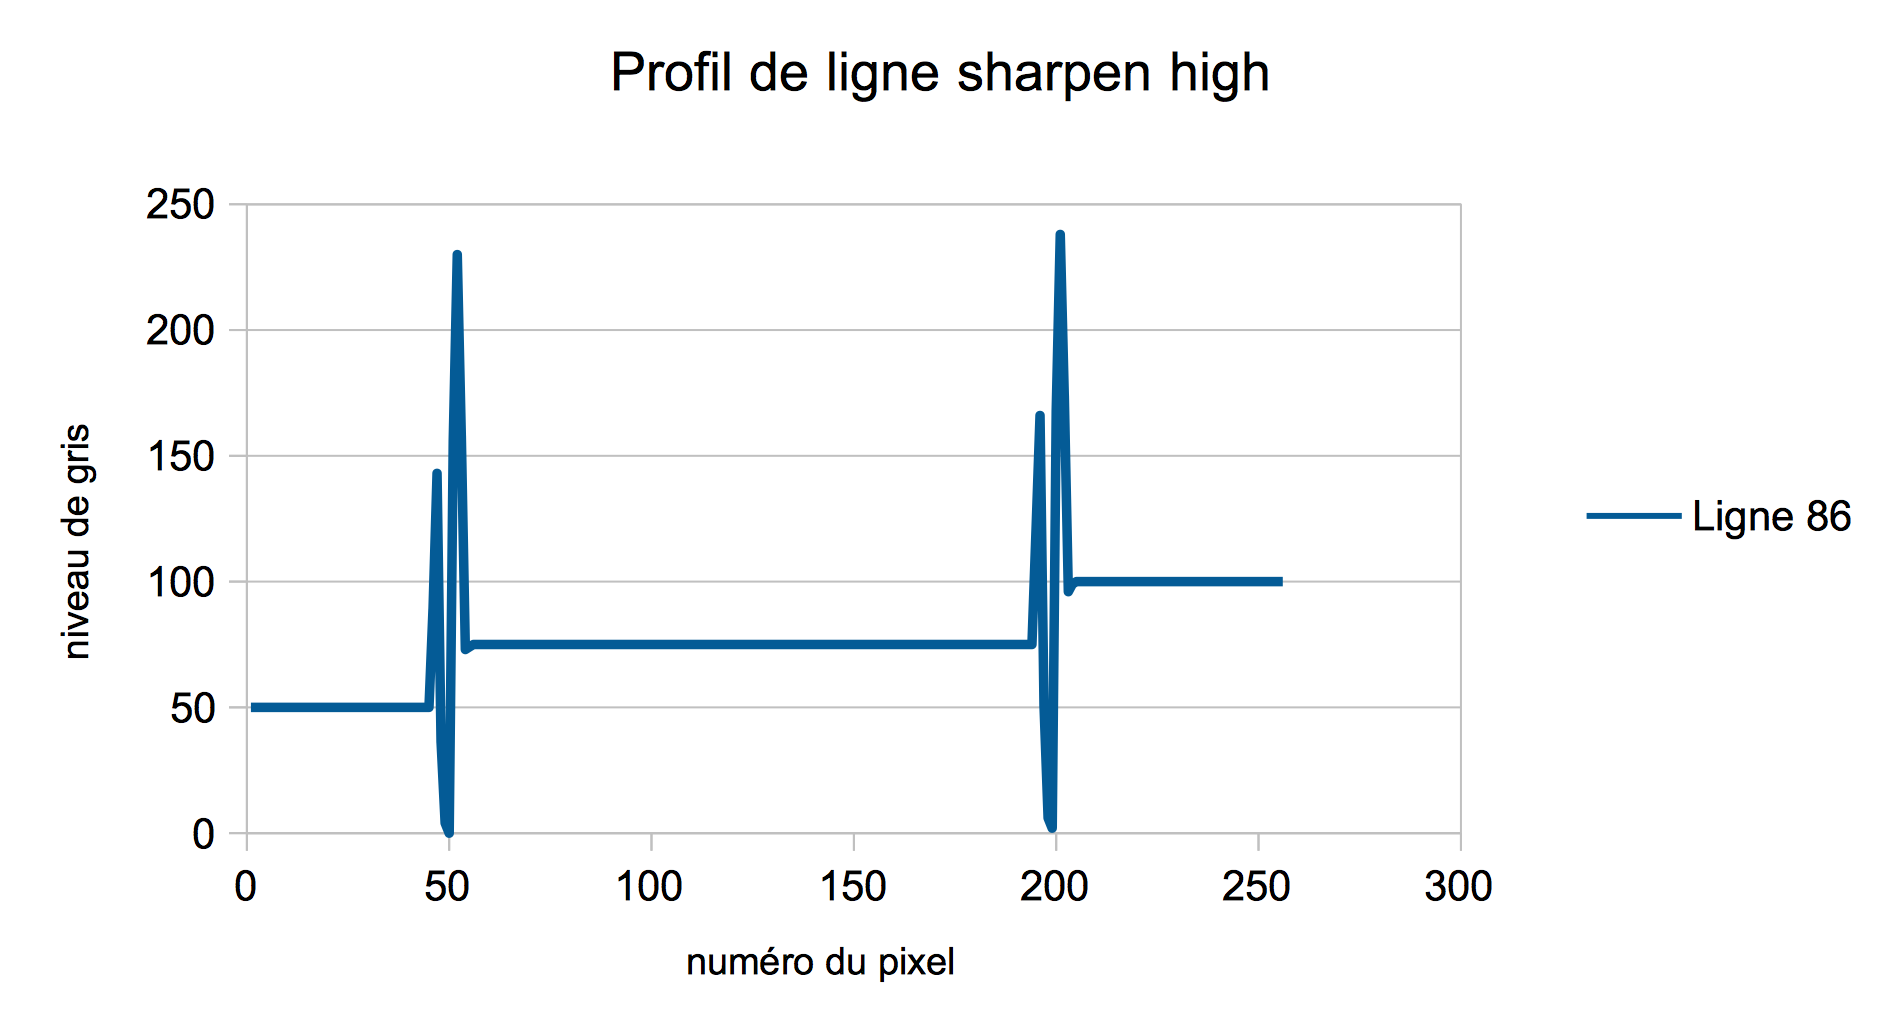
\includegraphics[height=7.5cm,width=15cm]{images/profillignesharpenhigh.png}
\caption{Profil de ligne de l'image mire_gris.tif auquel on a appliqué un filtre sharpen high}
\end{figure}

\newpage
\section{Détection de contours}
\addcontentsline{toc}{section}{Détection de contours}

Dans cette dernière partie, on veut mettre en évidence l'effet du filtre de Sobel. On réalisera 
à nouveau des profils de lignes sur les images bien connues, Connect_ok, Connect_L, Connect_D, Connect_B1
et enfin Connect_B2. Ensuite, on réalisera un filtrage de sobel en reprennant les profils de lignes. 


\begin{figure}[!h]
\centering
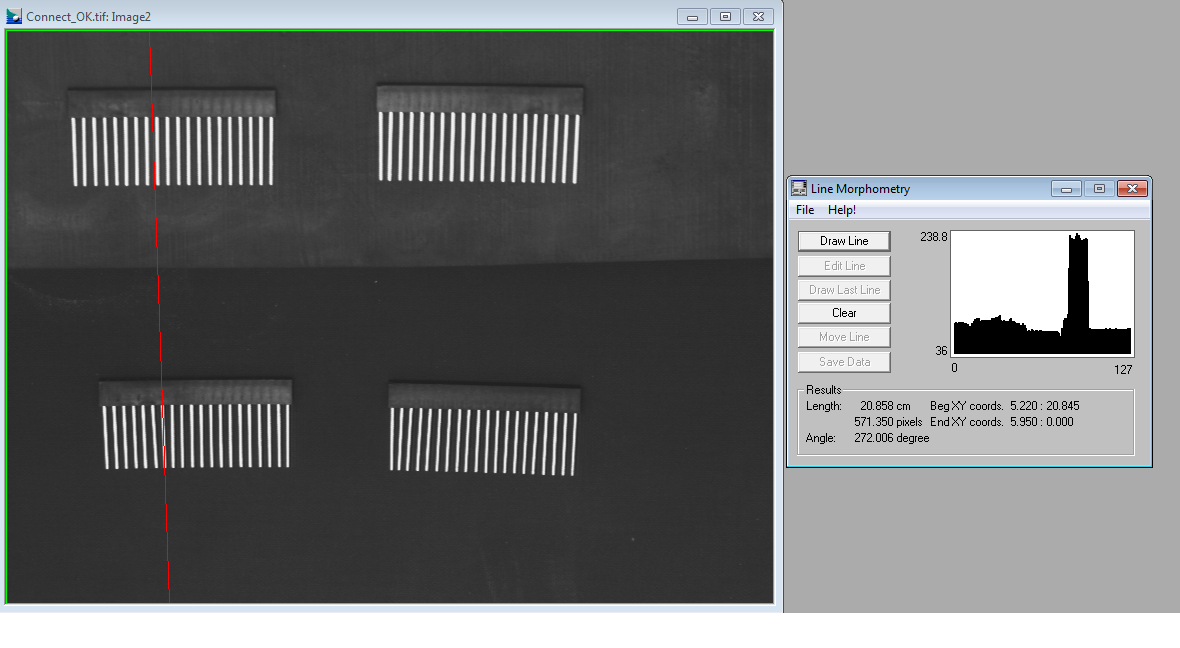
\includegraphics[height=7.5cm,width=15cm]{images/connectokline.png}
\caption{Profil de ligne de l'image Connect_ok.tif original}
\end{figure}

\begin{figure}[!h]
\centering
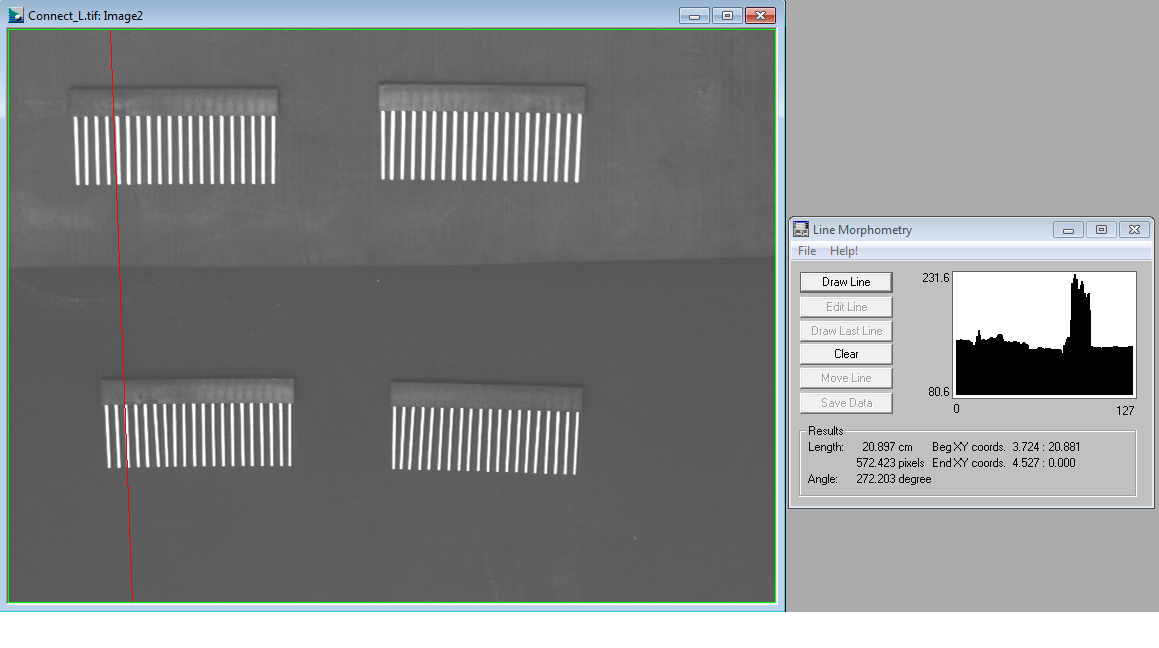
\includegraphics[height=7.5cm,width=15cm]{images/connectLline.png}
\caption{Profil de ligne de l'image Connect_L.tif original}
\end{figure}

\newpage
\begin{figure}[!h]
\centering
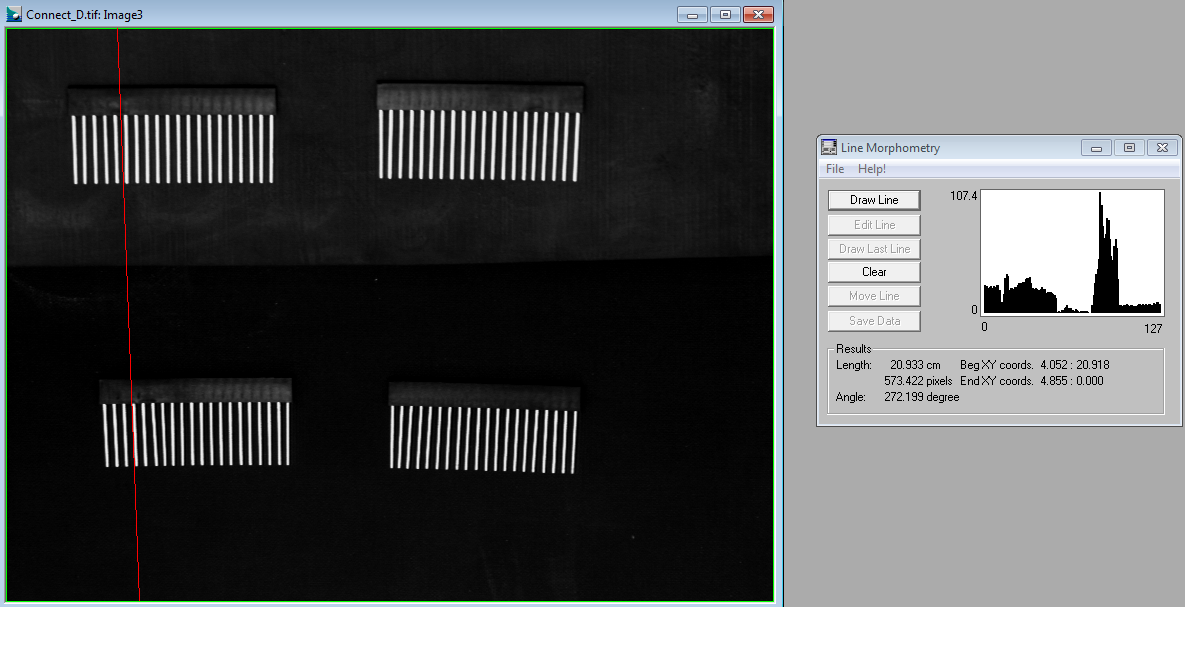
\includegraphics[height=7.5cm,width=15cm]{images/connectDline.png}
\caption{Profil de ligne de l'image Connect_D.tif original}
\end{figure}

\begin{figure}[!h]
\centering
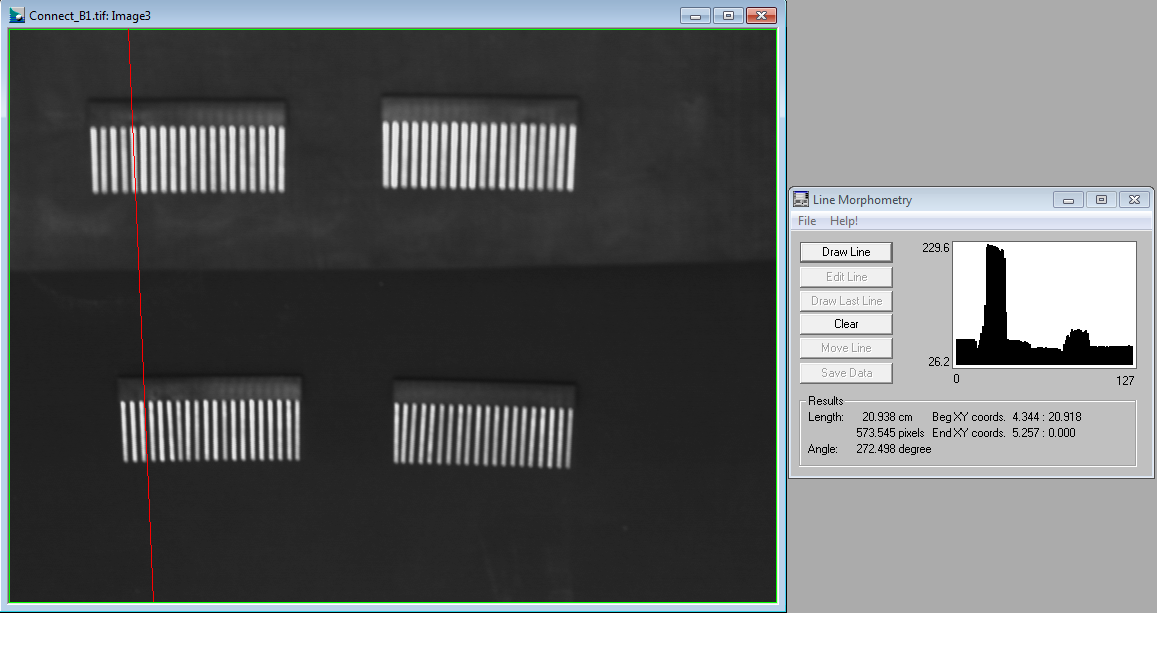
\includegraphics[height=7.5cm,width=15cm]{images/connectB1line.png}
\caption{Profil de ligne de l'image Connect_B1.tif original}
\end{figure}

\newpage
\begin{figure}[!h]
\centering
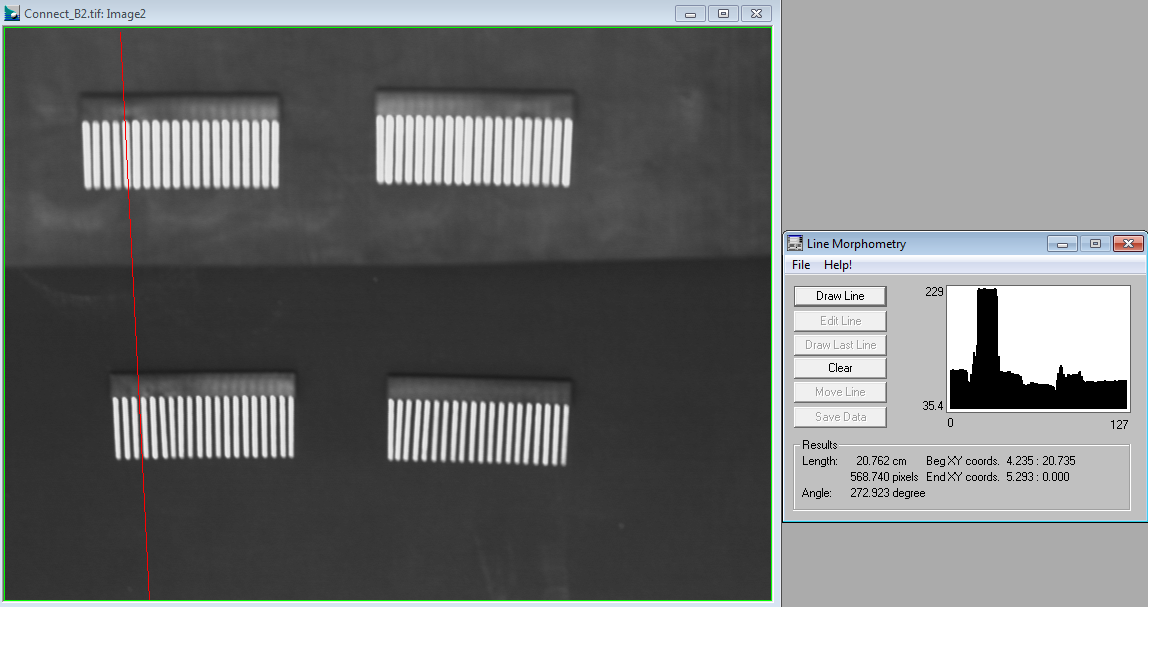
\includegraphics[height=7.5cm,width=15cm]{images/connectB2line.png}
\caption{Profil de ligne de l'image Connect_B2.tif original}
\end{figure}

On peut aisément observer les broches de ces connecteurs dans ces profils de colonnes qui correspondent aux pixels dont le niveau de gris est élevé. 

\begin{figure}[!h]
\centering
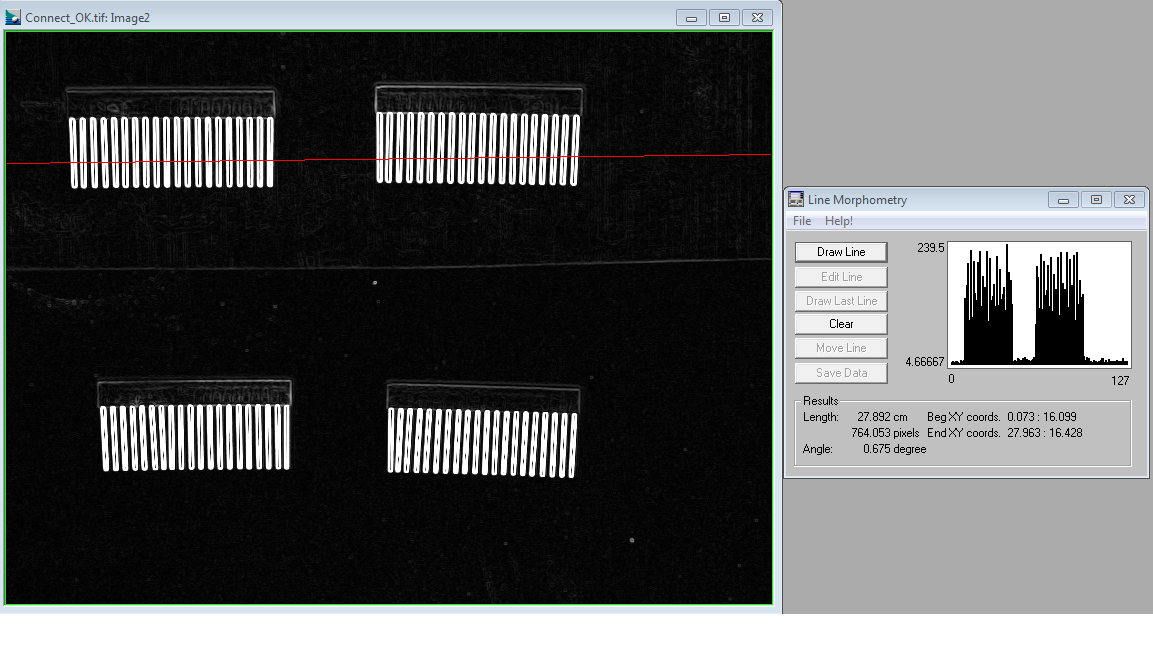
\includegraphics[height=7.5cm,width=15cm]{images/connectoklineSobel.png}
\caption{Profil de ligne de l'image Connect_ok.tif après filtrage avec Sobel}
\end{figure}

\newpage
\begin{figure}[!h]
\centering
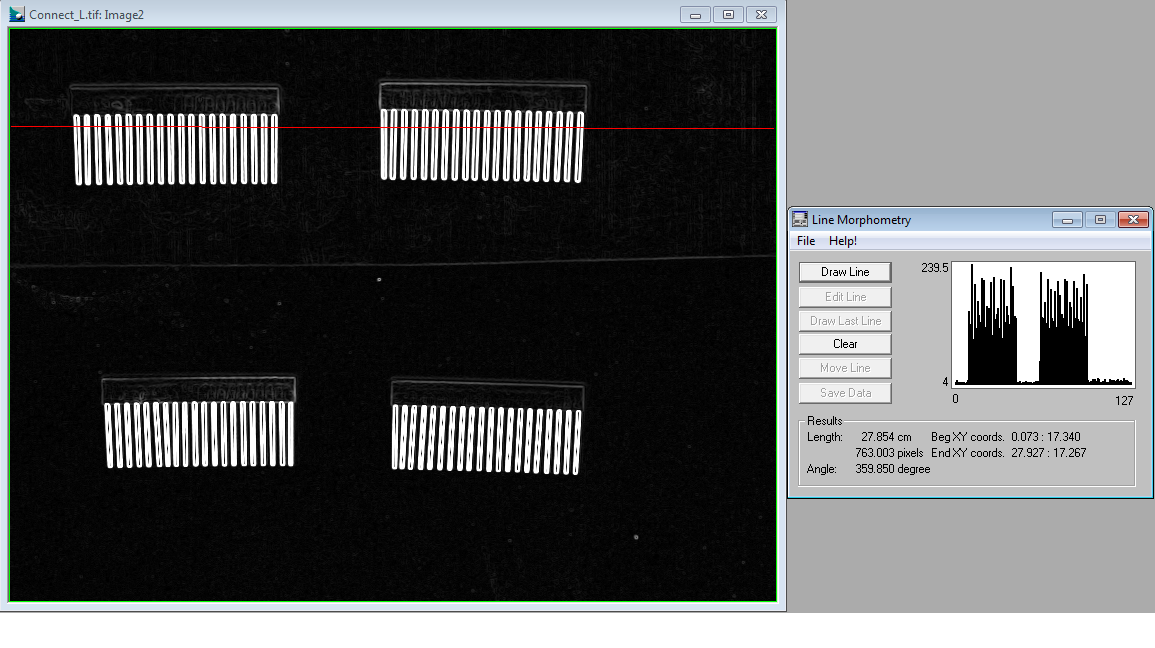
\includegraphics[height=7.5cm,width=15cm]{images/connectLlineSobel.png}
\caption{Profil de ligne de l'image Connect_L.tif après filtrage avec Sobel}
\end{figure}

\begin{figure}[!h]
\centering
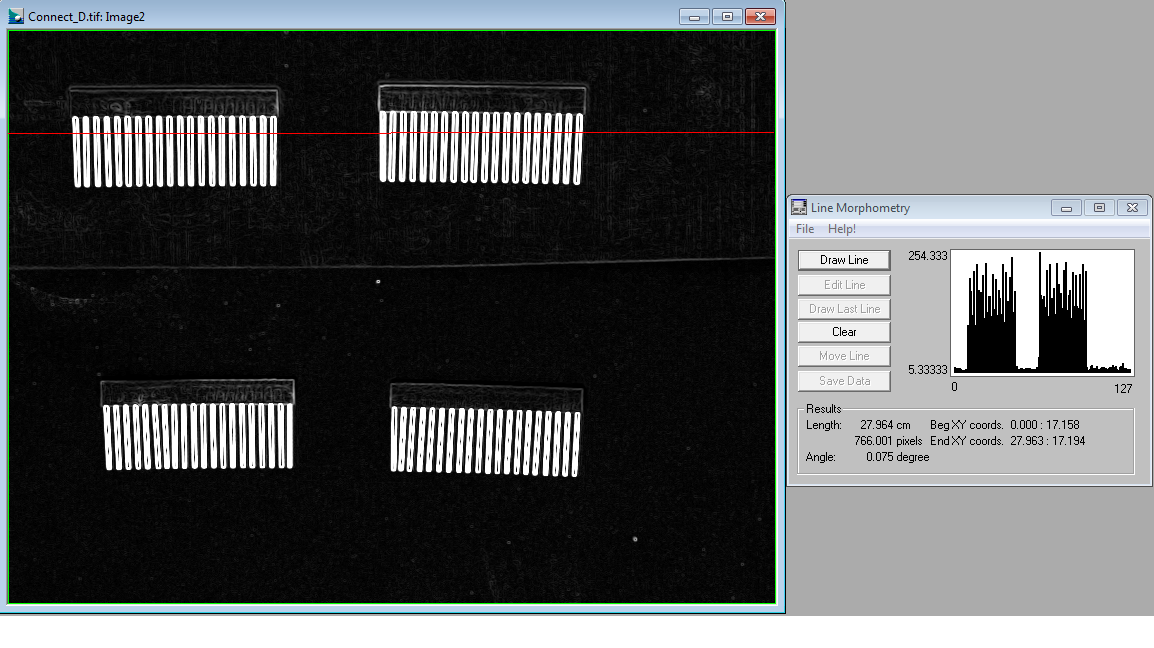
\includegraphics[height=7.5cm,width=15cm]{images/connectDlineSobel.png}
\caption{Profil de ligne de l'image Connect_D.tif après filtrage avec Sobel}
\end{figure}

\newpage
\begin{figure}[!h]
\centering
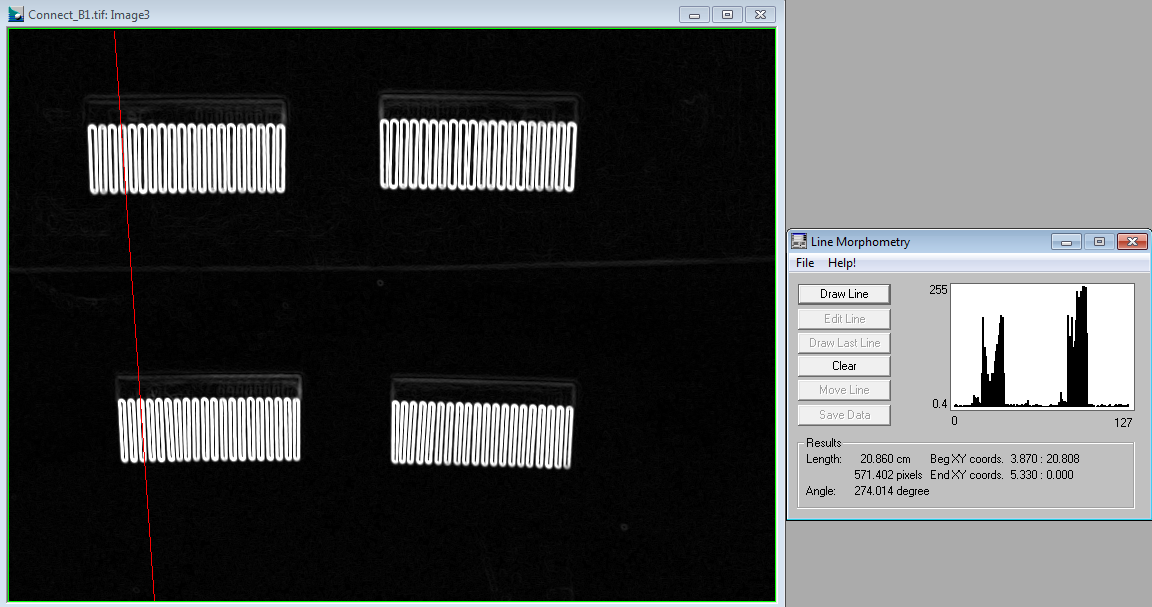
\includegraphics[height=7.5cm,width=15cm]{images/connectB1lineSobel.png}
\caption{Profil de ligne de l'image Connect_B1.tif après filtrage avec Sobel}
\end{figure}

\begin{figure}[!h]
\centering
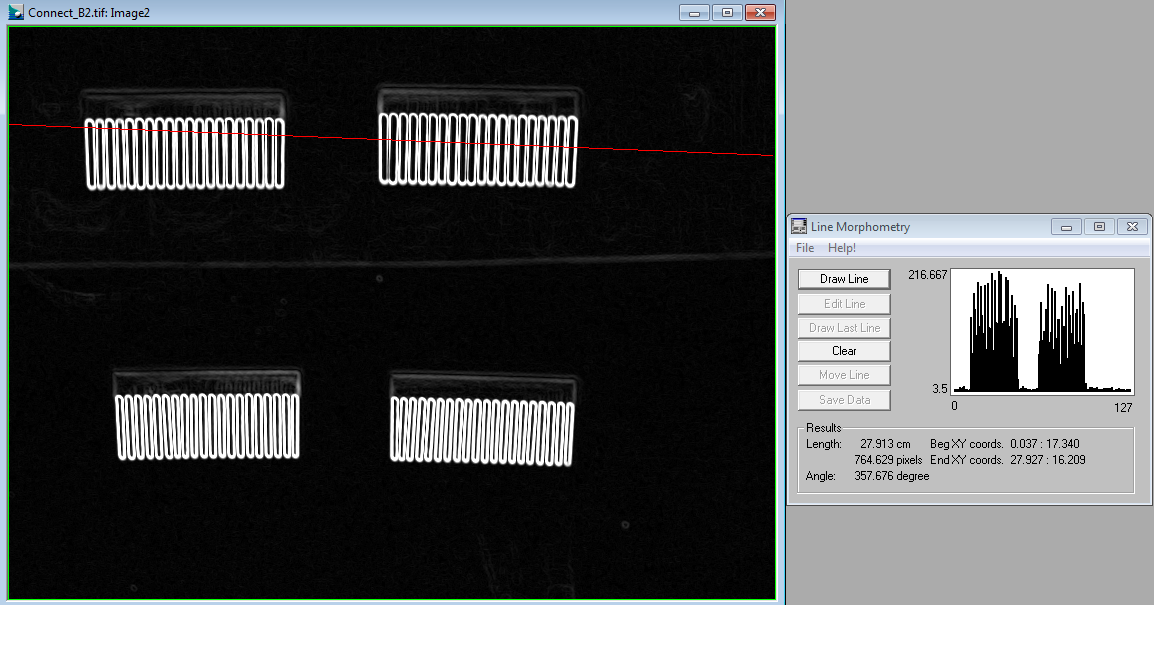
\includegraphics[height=7.5cm,width=15cm]{images/connectB2lineSobel.png}
\caption{Profil de ligne de l'image Connect_B2.tif après filtrage avec Sobel}
\end{figure}

Grâce à ces profils de ligne après filtrage avec Sobel, on remarque qu'il y a en fait deux pics par broches.

\newpage
\chapter{Troisième partie}
\addcontentsline{toc}{chapter}{Troisième partie}

\begin{center}
\large{
\textbf{Filtrage Morphologique}}
\end{center}

\section{Morphologie mathématique binaire}
\addcontentsline{toc}{section}{Morphologie mathématique binaire}


Pour cette dernière grande partie, on va travailler essentiellement sur l'image divers.tif.
Nous commençons par binariser cette image avant de pouvoir effectuer divers opérations morphologiques. 

Voici l'image binarisée. 

\begin{figure}[!h]
\centering
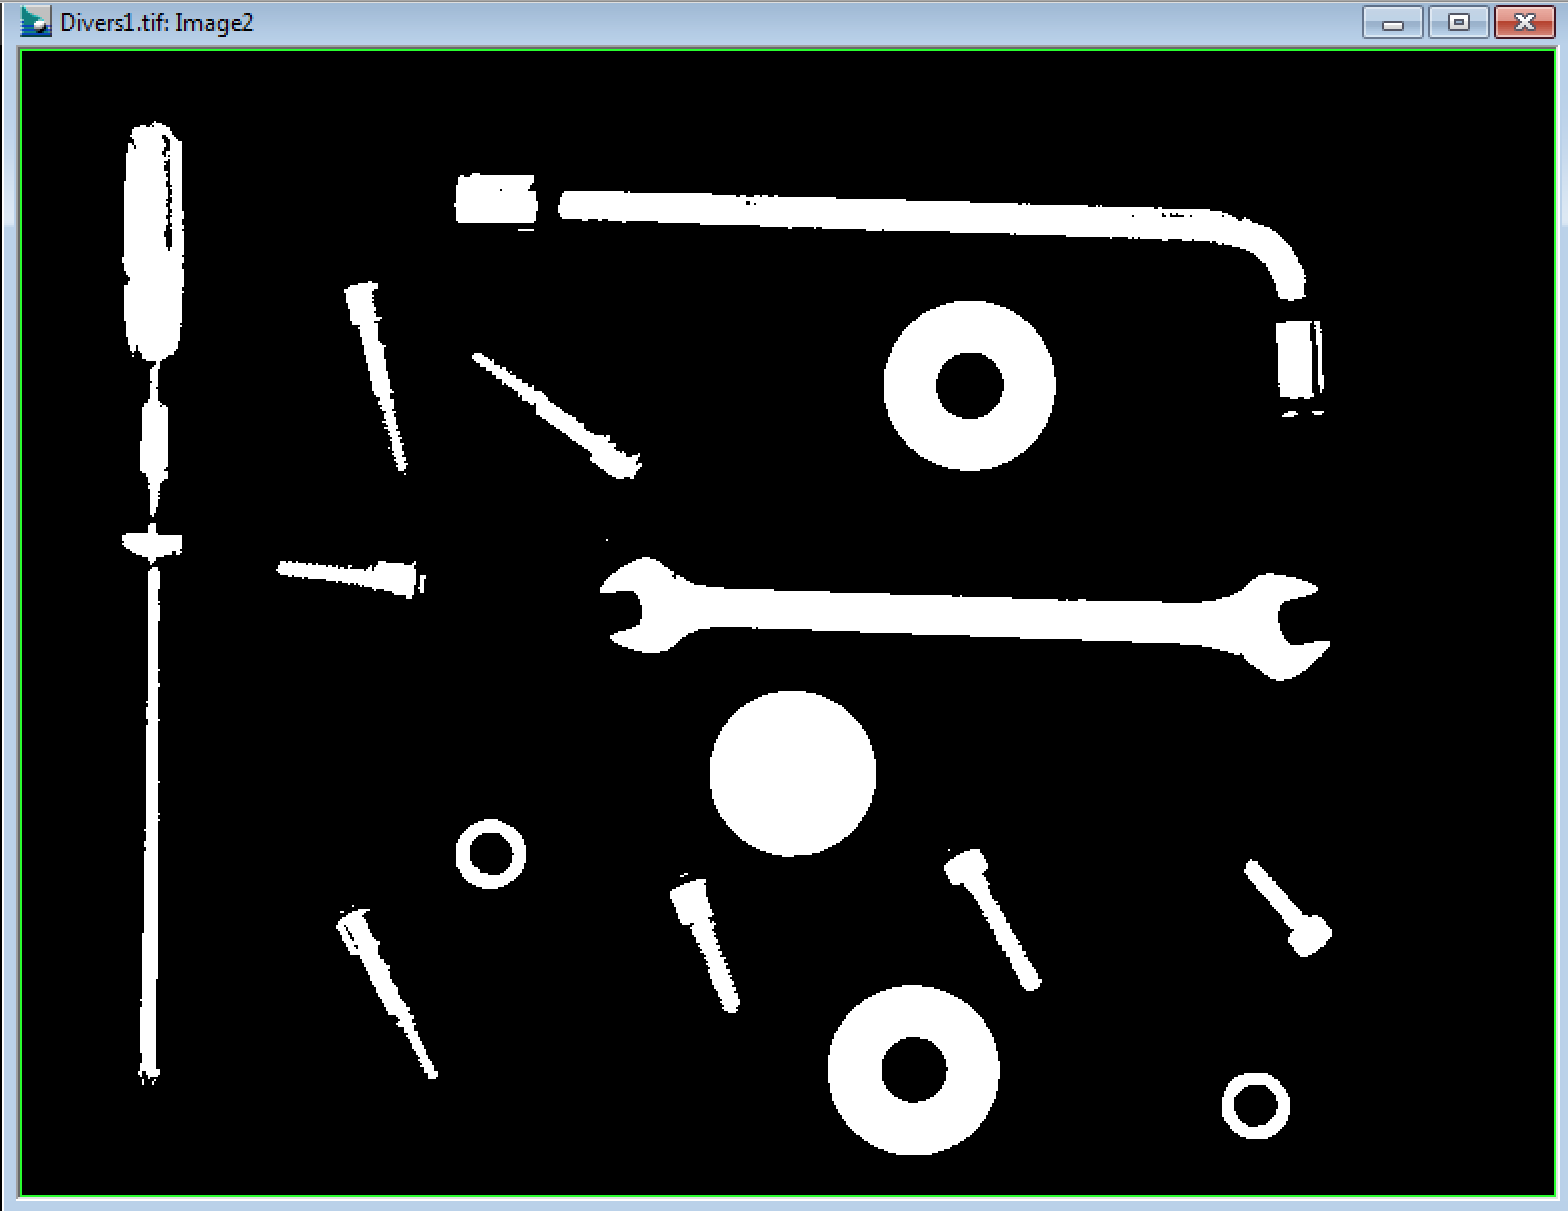
\includegraphics[height=7.5cm,width=15cm]{images/diversbinpes.png}
\caption{Image divers.tif binarisée}
\end{figure}

\newpage
Sur cette image on se propose maintenant de réaliser des dilatations et des erosions morphologiques. 
On obtient ce résultat. 

\begin{figure}[!h]
\centering
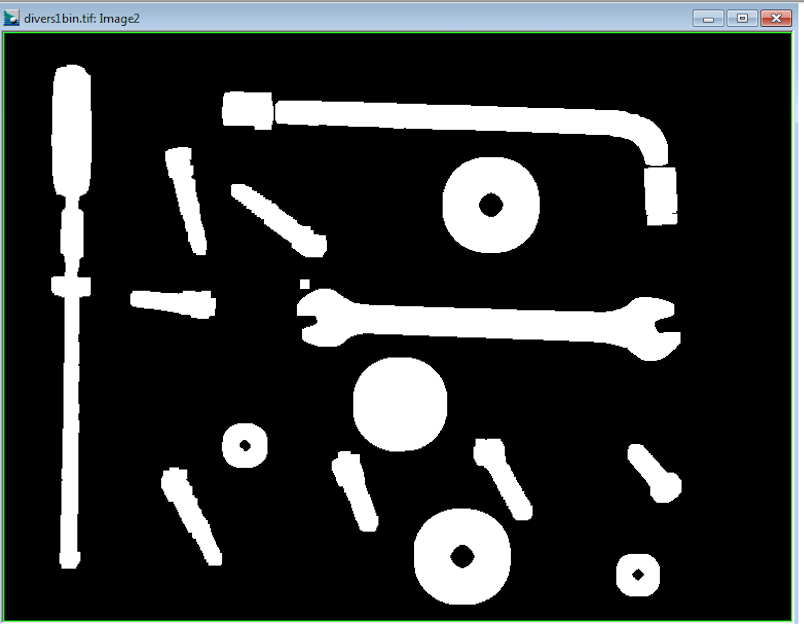
\includegraphics[height=5cm,width=5cm]{images/4dilates.png} \hfill
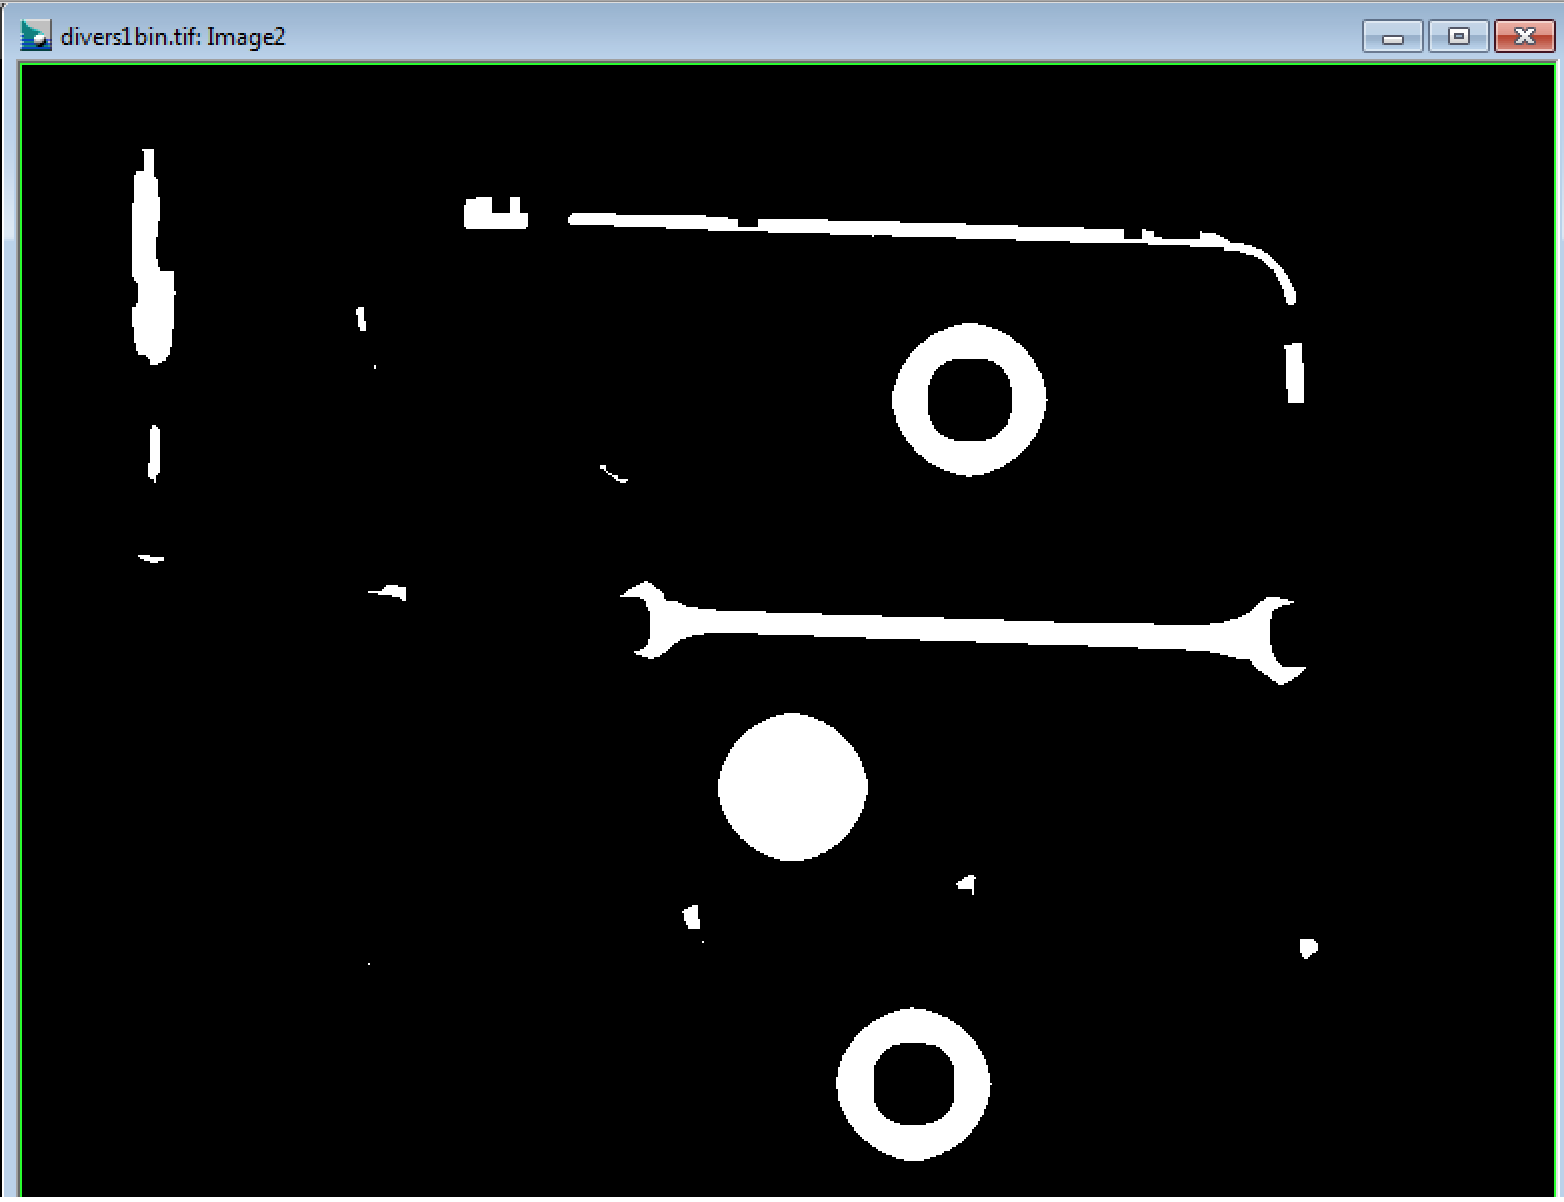
\includegraphics[height=5cm,width=5cm]{images/4erodes.png}
\caption{Image binarisée, quatre fois dilatée, quatres fois érodée}
\end{figure}

On remarque que les opérations de dilation et d'érosions morphologiques ne sont pas idempotentes.
De plus, on peut observer qu'on obtient le même résultat qu'en réalisant quatre dilatations ou quatre érosions, 
en appliquant une dilatations avec un élément structurant d'une taille quatre fois supérieure, ou une érosion avec
un élément struturant d'une taille quatre fois supérieure.

Voici le résultat après une dilatation en prenant un élément struturant de taille 4. 

\begin{figure}[!h]
\centering
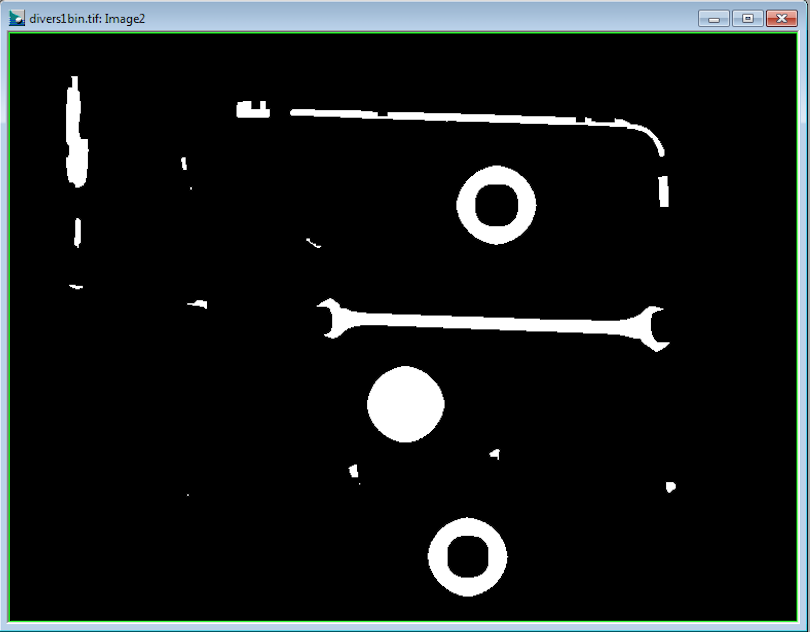
\includegraphics[height=7.5cm,width=15cm]{images/graydilatation.png}
\caption{Image divers binarisée dilaté avec un élément structurant de taille 4}
\end{figure}  

\newpage
On peut se séparer des pixels parasites avec les opérations open et close. 
En effet, on peut constater sur la figure suivante que nous n'avons plus de pixels parasites sur
l'image. 

\begin{figure}[!h]
\centering
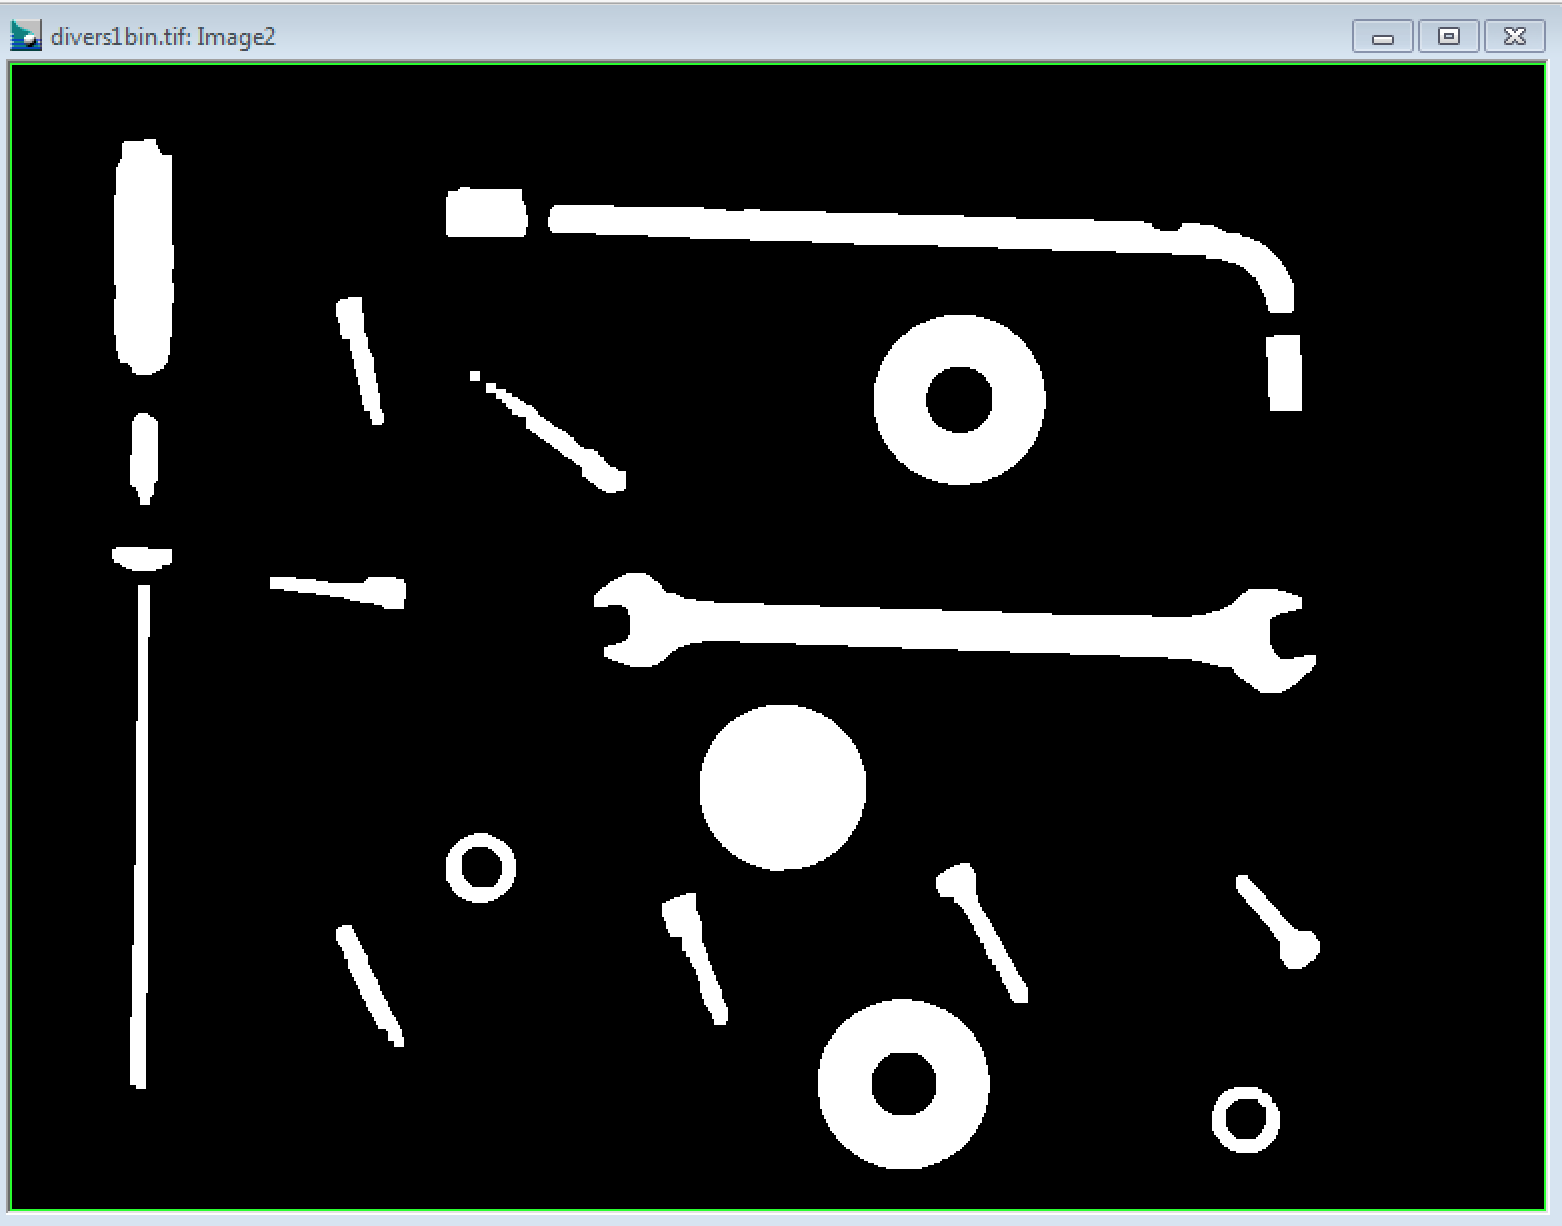
\includegraphics[height=5cm,width=5cm]{images/open.png} \hfill
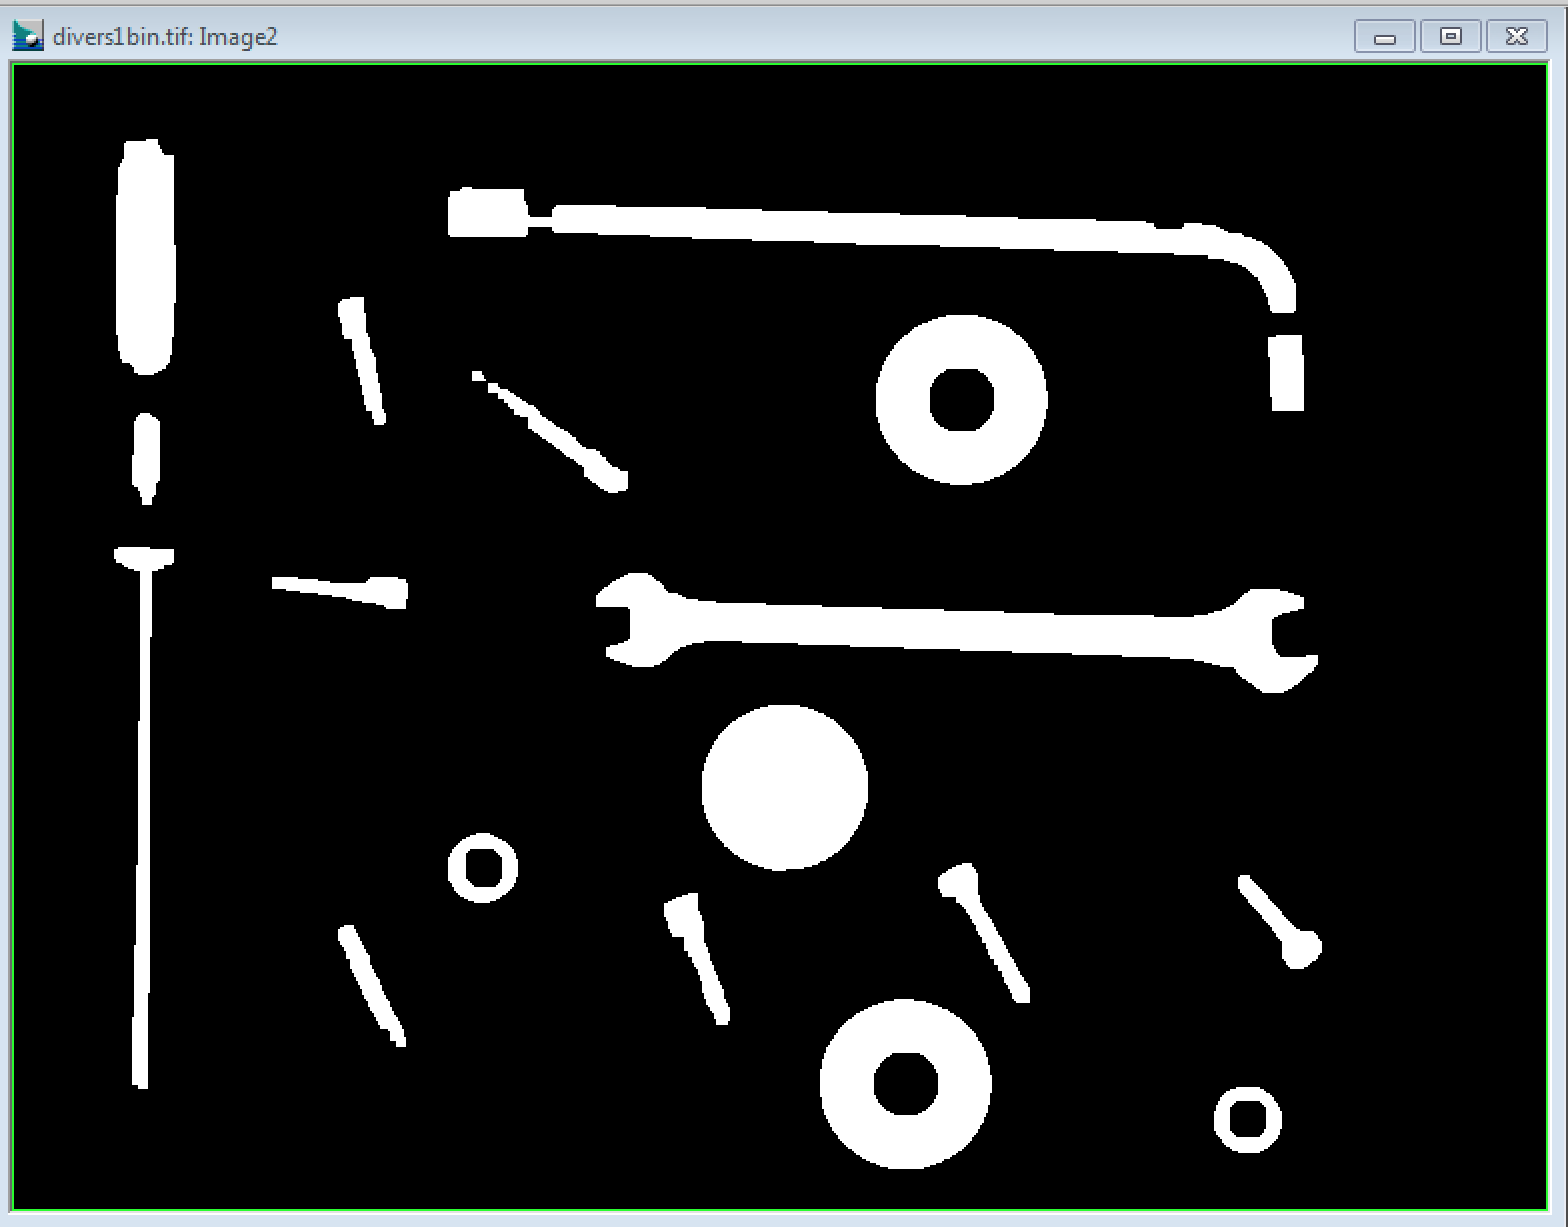
\includegraphics[height=5cm,width=5cm]{images/close.png}
\caption{Image divers binarisé sur laquelle on a respectivement réalisé une ouverture et une fermeture}
\end{figure}

Enfin, nous réalisons l'opération Outline qui nous donne les contours dans l'image. 

\begin{figure}[!h]
\centering
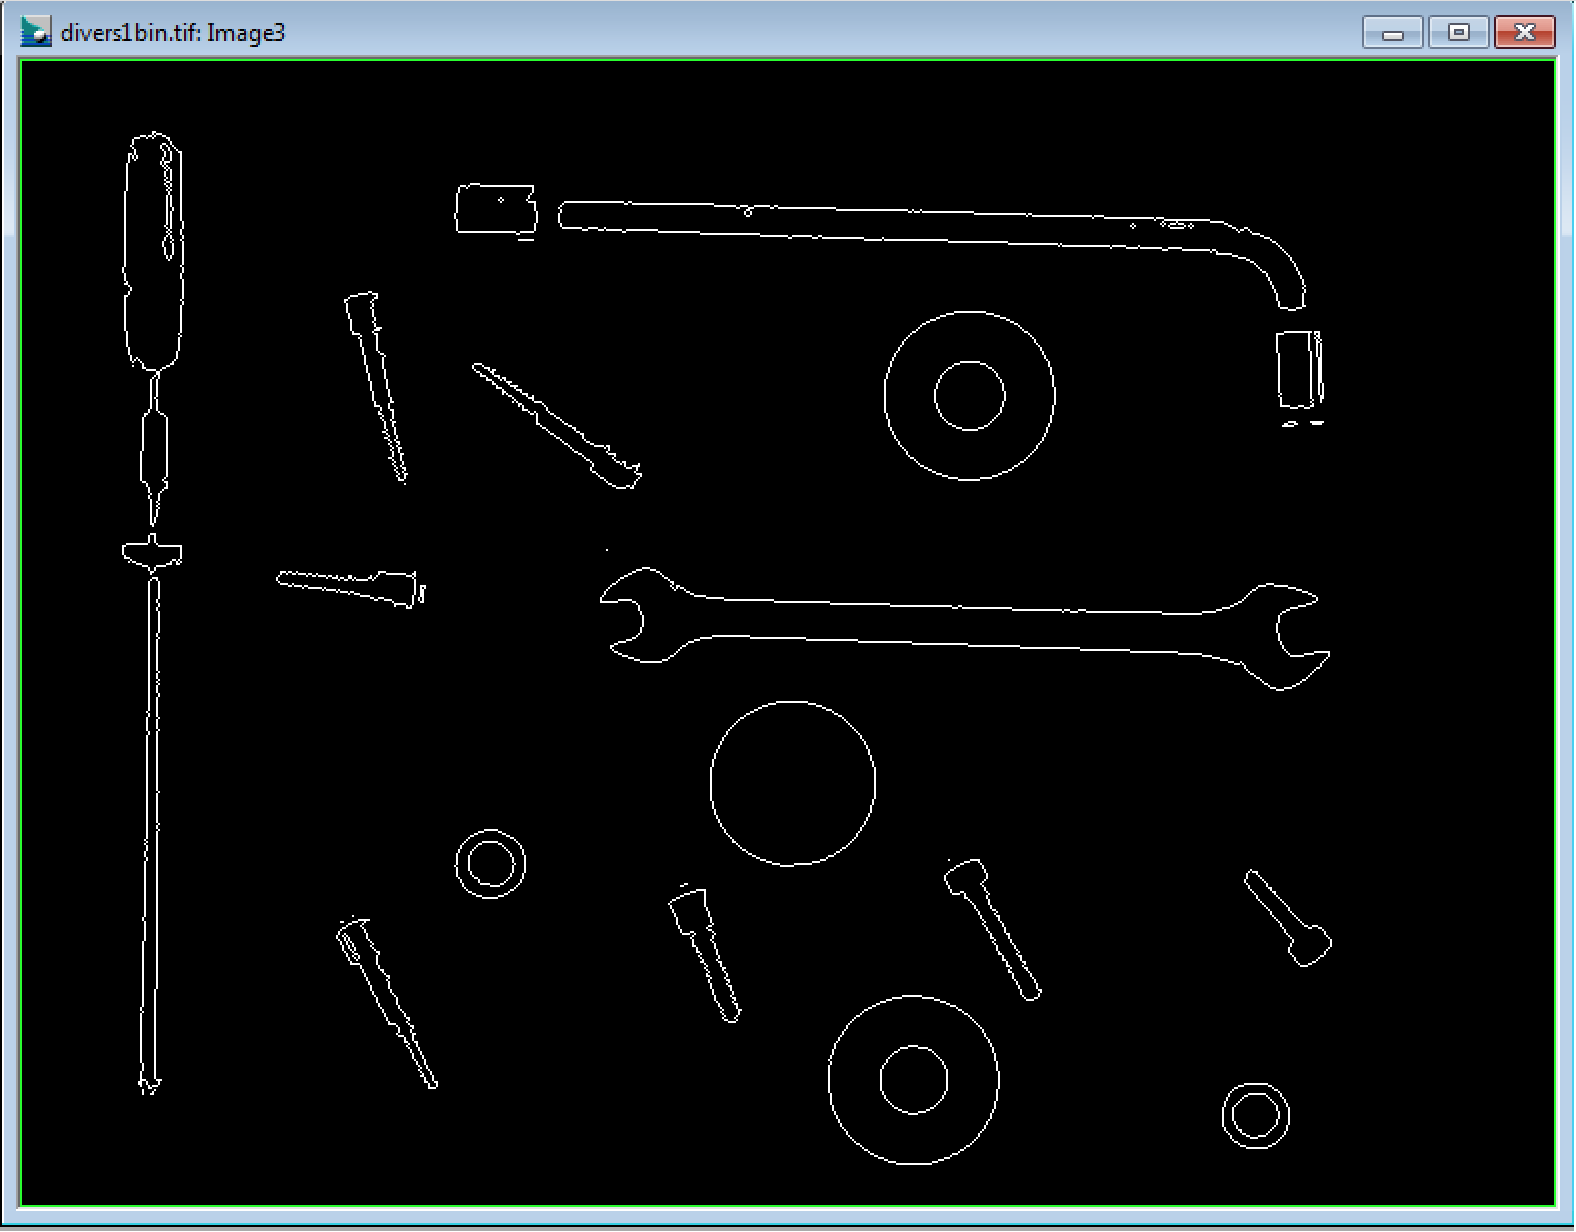
\includegraphics[height=7.5cm,width=15cm]{images/outline.png}
\caption{Image divers binarisé sur laquelle on a réalisé l'opération "outline"}
\end{figure}

\newpage
\section{Morphologie mathématique en niveau de gris}
\addcontentsline{toc}{section}{Morphologie mathématique en niveau de gris}

Voici nous donne les opérations d'érosion et de dilation en niveau gris sur l'image divers.

\begin{figure}[!h]
\centering
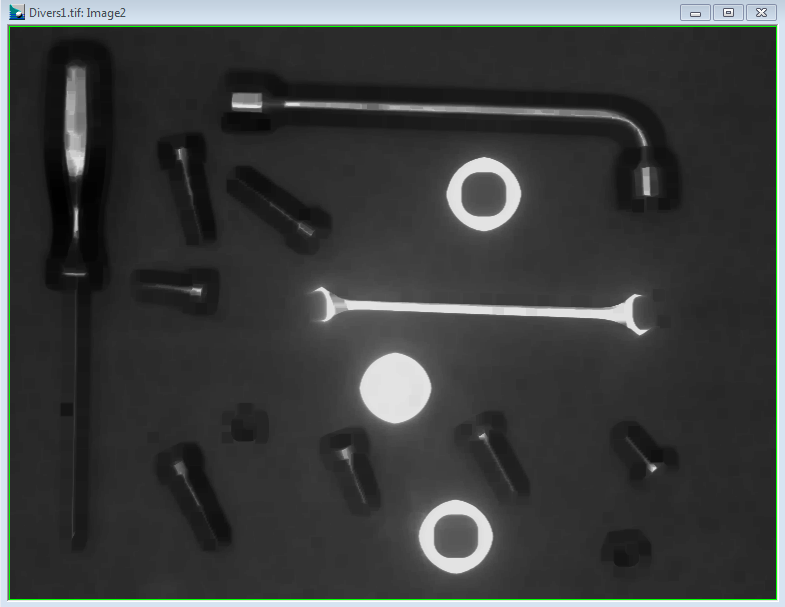
\includegraphics[height=5cm,width=5cm]{images/graylevelerode.png} \hfill
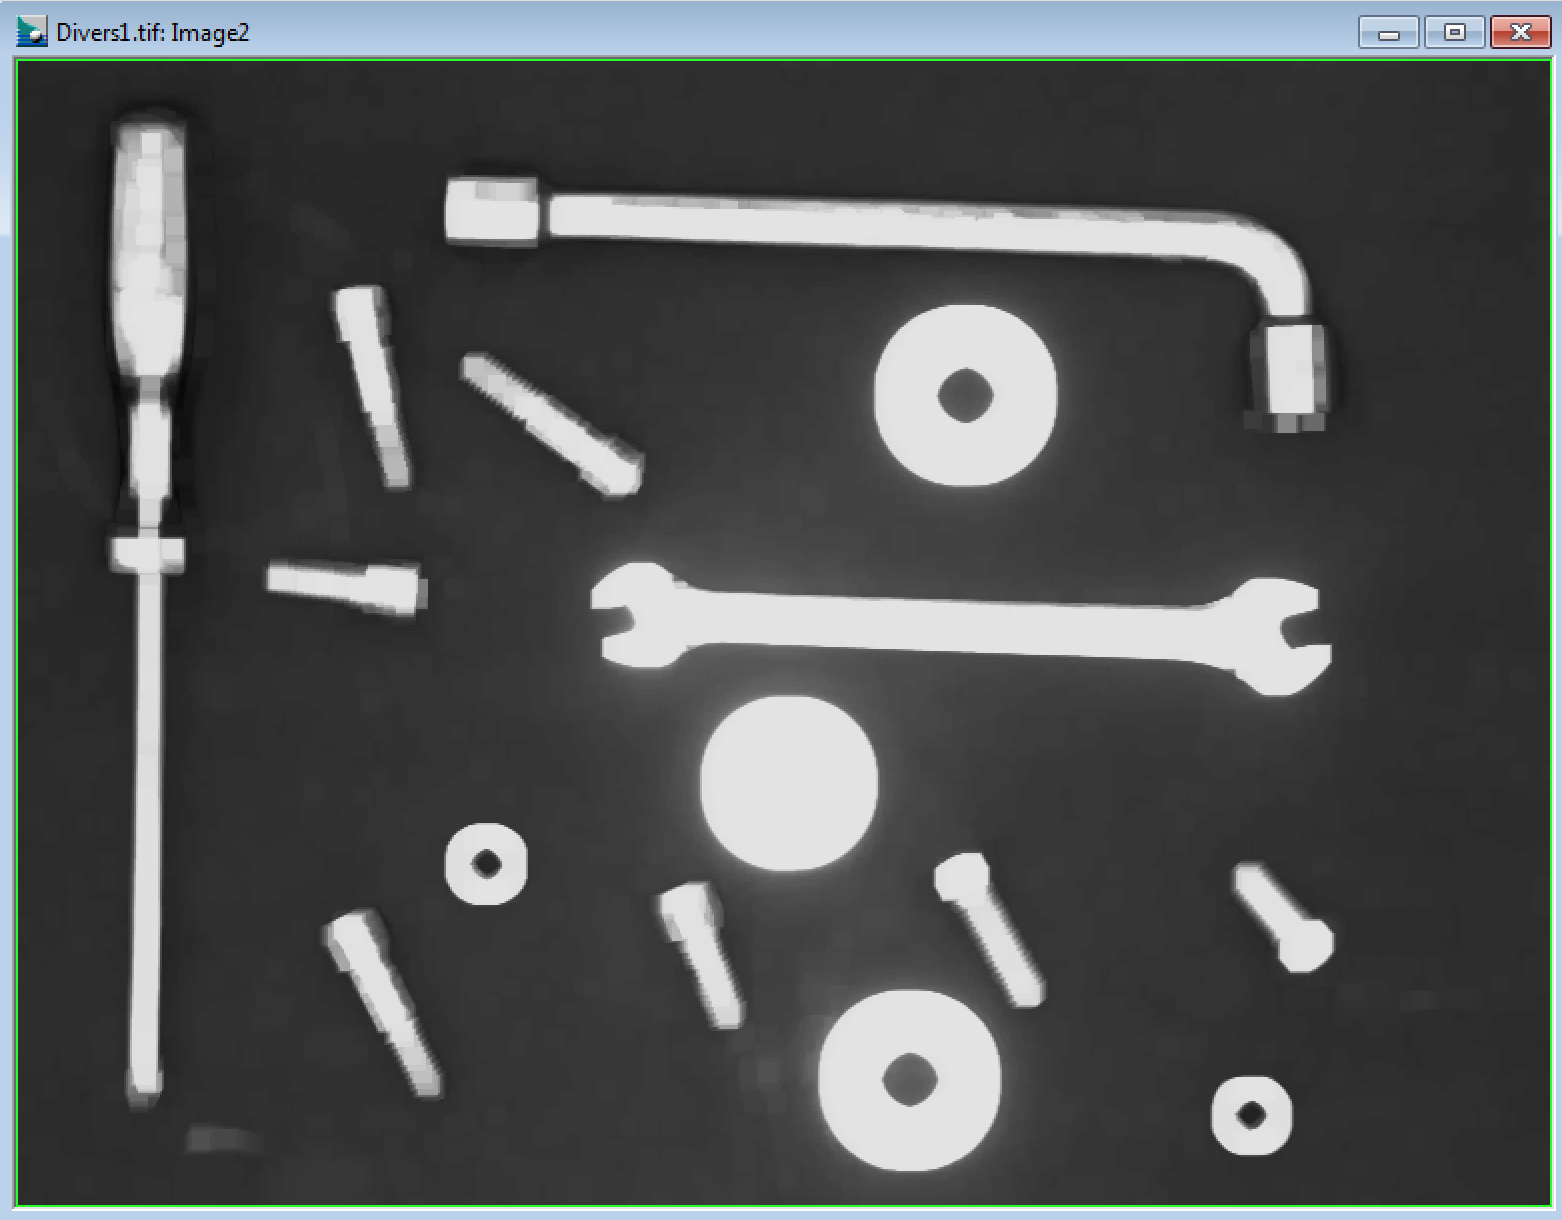
\includegraphics[height=5cm,width=5cm]{images/grayleveldilate.png}
\caption{Image divers en niveau de gris, érosions et dilatation}
\end{figure}

Voici pour finir la comparaison entre la détection de bord en niveau de gris par morphologie mathématique et
par sobel. 

\begin{figure}[!h]
\centering
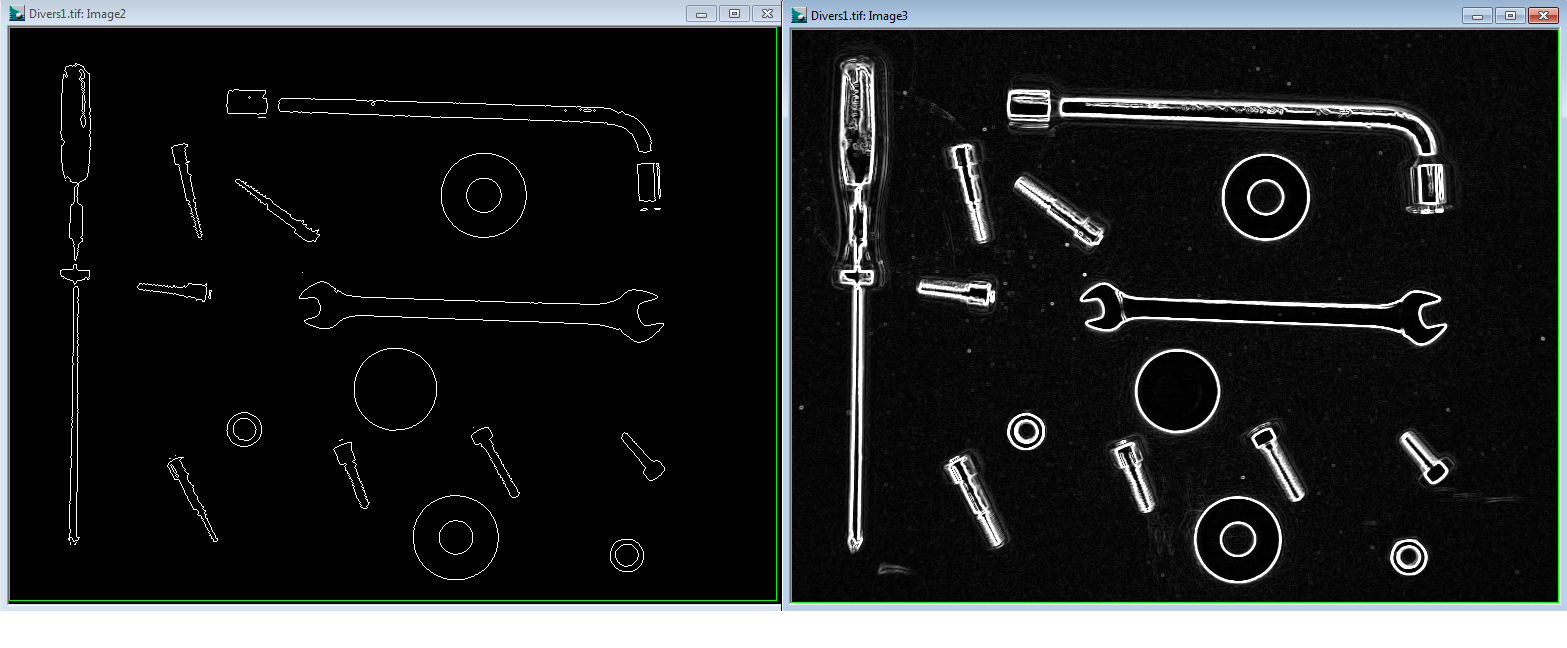
\includegraphics[height=7.5cm,width=15cm]{images/sobelVSMorphology.png}
\caption{Image divers en niveau de gris sur laquelle on compare la morphologie mathématique à Sobel}
\end{figure} 


\end{document}

